% ------------------------------------------------------------------------------
% Risk Modeller's Toolkit (RMTK) User Guide
%
% Authors:
% 	C. Casotto	- GEM Model Facility, Pavia, Italy
%
% Document distributed under the Common Creative License
% © GEM Foundation, Pavia, February 2014

%-------------------------------------------------------------------------------
%	LOAD PACKAGES
%-------------------------------------------------------------------------------
%%%%%%%%%%%%%%%%%%%%%%%%%%%%%%%%%%%%%%%%%
% The Legrand Orange Book
% LaTeX Template
% Version 1.4 (12/4/14)
%
% This template has been downloaded from:
% http://www.LaTeXTemplates.com
%
% Original author:
% Mathias Legrand (legrand.mathias@gmail.com)
%
% License:
% CC BY-NC-SA 3.0 (http://creativecommons.org/licenses/by-nc-sa/3.0/)
%
% Compiling this template:
% This template uses biber for its bibliography and makeindex for its index.
% When you first open the template, compile it from the command line with the 
% commands below to make sure your LaTeX distribution is configured correctly:
%
% 1) pdflatex rmtk-docs
% 1a) pdflatex -shell-escape rmtk-docs
% 2) makeindex rmtk-docs.idx -s StyleInd.ist
% 3) biber rmtk-docs
% 4  makeglossaries rmtk-docs
% 4) pdflatex rmtk-docs x 2
%
% After this, when you wish to update the bibliography/index use the appropriate
% command above and make sure to compile with pdflatex several times 
% afterwards to propagate your changes to the document.
%
% This template also uses a number of packages which may need to be
% updated to the newest versions for the template to compile. It is strongly
% recommended you update your LaTeX distribution if you have any
% compilation errors.
%
% Important note:
% Chapter heading images should have a 2:1 width:height ratio,
% e.g. 920px width and 460px height.
%
%%%%%%%%%%%%%%%%%%%%%%%%%%%%%%%%%%%%%%%%%

%----------------------------------------------------------------------------------------
%	PACKAGES AND OTHER DOCUMENT CONFIGURATIONS
%----------------------------------------------------------------------------------------

\documentclass[11pt,fleqn]{book} % Default font size and left-justified equations

\usepackage[top=3cm,bottom=3cm,left=3.2cm,right=3.2cm,headsep=10pt,a4paper]{geometry} % Page margins

\usepackage{xcolor} % Required for specifying colors by name
\definecolor{ocre}{RGB}{243,102,25} % Define the orange color used for highlighting throughout the book

% Font Settings
\usepackage{avant} % Use the Avantgarde font for headings
%\usepackage{times} % Use the Times font for headings
\usepackage{mathptmx} % Use the Adobe Times Roman as the default text font together with math symbols from the Sym­bol, Chancery and Com­puter Modern fonts

\usepackage{microtype} % Slightly tweak font spacing for aesthetics
\usepackage[utf8]{inputenc} % Required for including letters with accents
\usepackage[T1]{fontenc} % Use 8-bit encoding that has 256 glyphs

% Bibliography
\usepackage{csquotes}
\usepackage[style=alphabetic,
            sorting=nyt,
            sortcites=true,
            natbib=true,
            style=authoryear,
            maxcitenames=2,
            maxbibnames=100,
            autopunct=true,
            babel=hyphen,
            hyperref=true,
            doi=true,
            abbreviate=false,
            backref=true,
            backend=biber,
	    	uniquename=false,
	    	uniquelist=false]{biblatex}
\addbibresource{./bibliography/rmtk.bib} % BibTeX bibliography file
\defbibheading{bibempty}{}

% Figure caption settings
\usepackage[textfont=it,margin=10pt,font=small,labelfont=bf,labelsep=endash]{caption}
\usepackage{subcaption}
\usepackage{rotating}

% Table - colors from
\usepackage{verbatim}
\usepackage{color, colortbl}
\definecolor{almond}{rgb}{0.94, 0.87, 0.8}
\definecolor{ashgrey}{rgb}{0.7, 0.75, 0.71}
\definecolor{anti-flashwhite}{rgb}{0.95, 0.95, 0.96}
\definecolor{airforceblue}{rgb}{0.36, 0.54, 0.66}

% Index
\usepackage{calc} % For simpler calculation - used for spacing the index letter headings correctly
\usepackage{makeidx} % Required to make an index
% \setcounter{tocdepth}{3}    % entries down to \subsubsections in the TOC
\makeindex % Tells LaTeX to create the files required for indexing

\usepackage{todonotes}
\usepackage{geometry}
\usepackage{marginnote}

%
% Package to create a glossary - It must be uploaded after hyperref
% to produce the glossary: makeglossaries OQB
\usepackage[acronym,nonumberlist,style=altlist]{glossaries}
\glstoctrue
\makeglossaries

% package for bold symbols
\usepackage{bm}

% for better looking tables
\usepackage{ctable}
\usepackage{microtype}

% for listing Python code
\usepackage{listings}

%
%----------------------------------------------------------------------------------------
% Trees
%\usepackage[pdf]{pstricks}
%\usepackage{auto-pst-pdf}
%\usepackage{pst-tree}
%


%-------------------------------------------------------------------------------
% Insert the structure.tex file which contains the majority of the structure 
% behind the template
%----------------------------------------------------------------------------------------
%	VARIOUS REQUIRED PACKAGES
%----------------------------------------------------------------------------------------

\usepackage{titlesec} % Allows customization of titles

\usepackage{graphicx} % Required for including pictures
\graphicspath{{Pictures/}} % Specifies the directory where pictures are stored

\usepackage{tikz} % Required for drawing custom shapes

\usepackage[english]{babel} % English language/hyphenation

\usepackage{enumitem} % Customize lists
\setlist{nolistsep} % Reduce spacing between bullet points and numbered lists

\usepackage{booktabs} % Required for nicer horizontal rules in tables

\usepackage{eso-pic} % Required for specifying an image background in the title page
\usepackage{fancyvrb} % Verbatim environment
\usepackage{pdfpages} % Needed to load .pdf pages

%----------------------------------------------------------------------------------------
%	MAIN TABLE OF CONTENTS
%----------------------------------------------------------------------------------------

\usepackage{titletoc} % Required for manipulating the table of contents

\contentsmargin{0cm} % Removes the default margin
% Chapter text styling
\titlecontents{chapter}[1.25cm] % Indentation
{\addvspace{15pt}\large\sffamily\bfseries} % Spacing and font options for chapters
{\color{ocre!60}\contentslabel[\Large\thecontentslabel]{1.25cm}\color{ocre}} % Chapter number
{}  
{\color{ocre!60}\normalsize\sffamily\bfseries\;\titlerule*[.5pc]{.}\;\thecontentspage} % Page number
% Section text styling
\titlecontents{section}[1.25cm] % Indentation
{\addvspace{5pt}\sffamily\bfseries} % Spacing and font options for sections
{\contentslabel[\thecontentslabel]{1.25cm}} % Section number
{}
{\sffamily\hfill\color{black}\thecontentspage} % Page number
[]
% Subsection text styling
\titlecontents{subsection}[1.25cm] % Indentation
{\addvspace{1pt}\sffamily\small} % Spacing and font options for subsections
{\contentslabel[\thecontentslabel]{1.25cm}} % Subsection number
{}
{\sffamily\;\titlerule*[.5pc]{.}\;\thecontentspage} % Page number
[] 

%----------------------------------------------------------------------------------------
%	MINI TABLE OF CONTENTS IN CHAPTER HEADS
%----------------------------------------------------------------------------------------

% Section text styling
\titlecontents{lsection}[0em] % Indendating
{\footnotesize\sffamily} % Font settings
{}
{}
{}

% Subsection text styling
\titlecontents{lsubsection}[.5em] % Indentation
{\normalfont\footnotesize\sffamily} % Font settings
{}
{}
{}
 
%----------------------------------------------------------------------------------------
%	PAGE HEADERS
%----------------------------------------------------------------------------------------

\usepackage{fancyhdr} % Required for header and footer configuration

\pagestyle{fancy}
\renewcommand{\chaptermark}[1]{\markboth{\sffamily\normalsize\bfseries\chaptername\ \thechapter.\ #1}{}} % Chapter text font settings
\renewcommand{\sectionmark}[1]{\markright{\sffamily\normalsize\thesection\hspace{5pt}#1}{}} % Section text font settings
\fancyhf{} \fancyhead[LE,RO]{\sffamily\normalsize\thepage} % Font setting for the page number in the header
\fancyhead[LO]{\rightmark} % Print the nearest section name on the left side of odd pages
\fancyhead[RE]{\leftmark} % Print the current chapter name on the right side of even pages
\renewcommand{\headrulewidth}{0.5pt} % Width of the rule under the header
\addtolength{\headheight}{2.5pt} % Increase the spacing around the header slightly
\renewcommand{\footrulewidth}{0pt} % Removes the rule in the footer
\fancypagestyle{plain}{\fancyhead{}\renewcommand{\headrulewidth}{0pt}} % Style for when a plain pagestyle is specified

% Removes the header from odd empty pages at the end of chapters
\makeatletter
\renewcommand{\cleardoublepage}{
\clearpage\ifodd\c@page\else
\hbox{}
\vspace*{\fill}
\thispagestyle{empty}
\newpage
\fi}

%----------------------------------------------------------------------------------------
%	THEOREM STYLES
%----------------------------------------------------------------------------------------

\usepackage{amsmath,amsfonts,amssymb,amsthm} % For math equations, theorems, symbols, etc

\newcommand{\intoo}[2]{\mathopen{]}#1\,;#2\mathclose{[}}
\newcommand{\ud}{\mathop{\mathrm{{}d}}\mathopen{}}
\newcommand{\intff}[2]{\mathopen{[}#1\,;#2\mathclose{]}}
\newtheorem{notation}{Notation}[chapter]

%%%%%%%%%%%%%%%%%%%%%%%%%%%%%%%%%%%%%%%%%%%%%%%%%%%%%%%%%%%%%%%%%%%%%%%%%%%
%%%%%%%%%%%%%%%%%%%% dedicated to boxed/framed environements %%%%%%%%%%%%%%
%%%%%%%%%%%%%%%%%%%%%%%%%%%%%%%%%%%%%%%%%%%%%%%%%%%%%%%%%%%%%%%%%%%%%%%%%%%
\newtheoremstyle{ocrenumbox}% % Theorem style name
{0pt}% Space above
{0pt}% Space below
{\normalfont}% % Body font
{}% Indent amount
{\small\bf\sffamily\color{ocre}}% % Theorem head font
{\;}% Punctuation after theorem head
{0.25em}% Space after theorem head
{\small\sffamily\color{ocre}\thmname{#1}\nobreakspace\thmnumber{\@ifnotempty{#1}{}\@upn{#2}}% Theorem text (e.g. Theorem 2.1)
\thmnote{\nobreakspace\the\thm@notefont\sffamily\bfseries\color{black}---\nobreakspace#3.}} % Optional theorem note
\renewcommand{\qedsymbol}{$\blacksquare$}% Optional qed square

\newtheoremstyle{blacknumex}% Theorem style name
{5pt}% Space above
{5pt}% Space below
{\normalfont}% Body font
{} % Indent amount
{\small\bf\sffamily}% Theorem head font
{\;}% Punctuation after theorem head
{0.25em}% Space after theorem head
{\small\sffamily{\tiny\ensuremath{\blacksquare}}\nobreakspace\thmname{#1}\nobreakspace\thmnumber{\@ifnotempty{#1}{}\@upn{#2}}% Theorem text (e.g. Theorem 2.1)
\thmnote{\nobreakspace\the\thm@notefont\sffamily\bfseries---\nobreakspace#3.}}% Optional theorem note

\newtheoremstyle{blacknumbox} % Theorem style name
{0pt}% Space above
{0pt}% Space below
{\normalfont}% Body font
{}% Indent amount
{\small\bf\sffamily}% Theorem head font
{\;}% Punctuation after theorem head
{0.25em}% Space after theorem head
{\small\sffamily\thmname{#1}\nobreakspace\thmnumber{\@ifnotempty{#1}{}\@upn{#2}}% Theorem text (e.g. Theorem 2.1)
\thmnote{\nobreakspace\the\thm@notefont\sffamily\bfseries---\nobreakspace#3.}}% Optional theorem note

%%%%%%%%%%%%%%%%%%%%%%%%%%%%%%%%%%%%%%%%%%%%%%%%%%%%%%%%%%%%%%%%%%%%%%%%%%%
%%%%%%%%%%%%% dedicated to non-boxed/non-framed environements %%%%%%%%%%%%%
%%%%%%%%%%%%%%%%%%%%%%%%%%%%%%%%%%%%%%%%%%%%%%%%%%%%%%%%%%%%%%%%%%%%%%%%%%%
\newtheoremstyle{ocrenum}% % Theorem style name
{5pt}% Space above
{5pt}% Space below
{\normalfont}% % Body font
{}% Indent amount
{\small\bf\sffamily\color{ocre}}% % Theorem head font
{\;}% Punctuation after theorem head
{0.25em}% Space after theorem head
{\small\sffamily\color{ocre}\thmname{#1}\nobreakspace\thmnumber{\@ifnotempty{#1}{}\@upn{#2}}% Theorem text (e.g. Theorem 2.1)
\thmnote{\nobreakspace\the\thm@notefont\sffamily\bfseries\color{black}---\nobreakspace#3.}} % Optional theorem note
\renewcommand{\qedsymbol}{$\blacksquare$}% Optional qed square
\makeatother

% Defines the theorem text style for each type of theorem to one of the three styles above
\newcounter{dummy} 
\numberwithin{dummy}{section}
\theoremstyle{ocrenumbox}
\newtheorem{theoremeT}[dummy]{Theorem}
\newtheorem{problem}{Problem}[chapter]
\newtheorem{exerciseT}{Exercise}[chapter]
\theoremstyle{blacknumex}
\newtheorem{exampleT}{Example}[chapter]
\theoremstyle{blacknumbox}
\newtheorem{vocabulary}{Vocabulary}[chapter]
\newtheorem{definitionT}{Definition}[section]
\newtheorem{corollaryT}[dummy]{Corollary}
\theoremstyle{ocrenum}
\newtheorem{proposition}[dummy]{Proposition}

%----------------------------------------------------------------------------------------
%	DEFINITION OF COLORED BOXES
%----------------------------------------------------------------------------------------

\RequirePackage[framemethod=default]{mdframed} % Required for creating the theorem, definition, exercise and corollary boxes

% Theorem box
\newmdenv[skipabove=7pt,
skipbelow=7pt,
backgroundcolor=black!5,
linecolor=ocre,
innerleftmargin=5pt,
innerrightmargin=5pt,
innertopmargin=5pt,
leftmargin=0cm,
rightmargin=0cm,
innerbottommargin=5pt]{tBox}

% Exercise box	  
\newmdenv[skipabove=7pt,
skipbelow=7pt,
rightline=false,
leftline=true,
topline=false,
bottomline=false,
backgroundcolor=ocre!10,
linecolor=ocre,
innerleftmargin=5pt,
innerrightmargin=5pt,
innertopmargin=5pt,
innerbottommargin=5pt,
leftmargin=0cm,
rightmargin=0cm,
linewidth=4pt]{eBox}	

% Definition box
\newmdenv[skipabove=7pt,
skipbelow=7pt,
rightline=false,
leftline=true,
topline=false,
bottomline=false,
linecolor=ocre,
innerleftmargin=5pt,
innerrightmargin=5pt,
innertopmargin=0pt,
leftmargin=0cm,
rightmargin=0cm,
linewidth=4pt,
innerbottommargin=0pt]{dBox}	

% Corollary box
\newmdenv[skipabove=7pt,
skipbelow=7pt,
rightline=false,
leftline=true,
topline=false,
bottomline=false,
linecolor=gray,
backgroundcolor=black!5,
innerleftmargin=5pt,
innerrightmargin=5pt,
innertopmargin=5pt,
leftmargin=0cm,
rightmargin=0cm,
linewidth=4pt,
innerbottommargin=5pt]{cBox}

% Creates an environment for each type of theorem and assigns it a theorem text style from the "Theorem Styles" section above and a colored box from above
\newenvironment{theorem}{\begin{tBox}\begin{theoremeT}}{\end{theoremeT}\end{tBox}}
\newenvironment{exercise}{\begin{eBox}\begin{exerciseT}}{\hfill{\color{ocre}\tiny\ensuremath{\blacksquare}}\end{exerciseT}\end{eBox}}				  
\newenvironment{definition}{\begin{dBox}\begin{definitionT}}{\end{definitionT}\end{dBox}}	
\newenvironment{example}{\begin{exampleT}}{\hfill{\tiny\ensuremath{\blacksquare}}\end{exampleT}}		
\newenvironment{corollary}{\begin{cBox}\begin{corollaryT}}{\end{corollaryT}\end{cBox}}	

%----------------------------------------------------------------------------------------
%	REMARK ENVIRONMENT
%----------------------------------------------------------------------------------------

\newenvironment{remark}{\par\vspace{10pt}\small % Vertical white space above the remark and smaller font size
\begin{list}{}{
\leftmargin=35pt % Indentation on the left
\rightmargin=25pt}\item\ignorespaces % Indentation on the right
\makebox[-2.5pt]{\begin{tikzpicture}[overlay]
\node[draw=ocre!60,line width=1pt,circle,fill=ocre!25,font=\sffamily\bfseries,inner sep=2pt,outer sep=0pt] at (-15pt,0pt){\textcolor{ocre}{R}};\end{tikzpicture}} % Orange R in a circle
\advance\baselineskip -1pt}{\end{list}\vskip5pt} % Tighter line spacing and white space after remark

%----------------------------------------------------------------------------------------
%	SECTION NUMBERING IN THE MARGIN
%----------------------------------------------------------------------------------------

\makeatletter
\renewcommand{\@seccntformat}[1]{\llap{\textcolor{ocre}{\csname the#1\endcsname}\hspace{1em}}}                    
\renewcommand{\section}{\@startsection{section}{1}{\z@}
{-4ex \@plus -1ex \@minus -.4ex}
{1ex \@plus.2ex }
{\normalfont\large\sffamily\bfseries}}
\renewcommand{\subsection}{\@startsection {subsection}{2}{\z@}
{-3ex \@plus -0.1ex \@minus -.4ex}
{0.5ex \@plus.2ex }
{\normalfont\sffamily\bfseries}}
\renewcommand{\subsubsection}{\@startsection {subsubsection}{3}{\z@}
{-2ex \@plus -0.1ex \@minus -.2ex}
{.2ex \@plus.2ex }
{\normalfont\small\sffamily\bfseries}}                        
\renewcommand\paragraph{\@startsection{paragraph}{4}{\z@}
{-2ex \@plus-.2ex \@minus .2ex}
{.1ex}
{\normalfont\small\sffamily\bfseries}}

%----------------------------------------------------------------------------------------
%	HYPERLINKS IN THE DOCUMENTS
%----------------------------------------------------------------------------------------

% For an unclear reason, the package should be loaded now and not later
\usepackage{hyperref}
\hypersetup{hidelinks,backref=true,pagebackref=true,hyperindex=true,colorlinks=false,breaklinks=true,urlcolor= ocre,bookmarks=true,bookmarksopen=false,pdftitle={Title},pdfauthor={Author}}

%----------------------------------------------------------------------------------------
%	CHAPTER HEADINGS
%----------------------------------------------------------------------------------------

% The set-up below should be (sadly) manually adapted to the overall margin page
% septup controlled by the geometry package loaded in the main.tex document. It
% is possible to implement below the dimensions used in the goemetry package
% (top,bottom,left,right)... TO BE DONE

\newcommand{\thechapterimage}{}
\newcommand{\chapterimage}[1]{\renewcommand{\thechapterimage}{#1}}

% Numbered chapters with mini tableofcontents
\def\thechapter{\arabic{chapter}}
\def\@makechapterhead#1{
\thispagestyle{empty}
{\centering \normalfont\sffamily
\ifnum \c@secnumdepth >\m@ne
\if@mainmatter
\startcontents
\begin{tikzpicture}[remember picture,overlay]
\node at (current page.north west)
{\begin{tikzpicture}[remember picture,overlay]
\node[anchor=north west,inner sep=0pt] at (0,0) {\includegraphics[width=\paperwidth]{\thechapterimage}};
%%%%%%%%%%%%%%%%%%%%%%%%%%%%%%%%%%%%%%%%%%%%%%%%%%%%%%%%%%%%%%%%%%%%%%%%%%%%%%%%%%%%%
% Commenting the 3 lines below removes the small contents box in the chapter heading
\fill[color=ocre!10!white,opacity=.6] (1cm,0) rectangle (8cm,-7cm);
\node[anchor=north west] at (1.1cm,.35cm) {\parbox[t][8cm][t]{6.5cm}{
    \huge\bfseries\flushleft \printcontents{l}{1}{\setcounter{tocdepth}{2}}}};
\draw[anchor=west] (5cm,-9cm) node [rounded corners=20pt,fill=ocre!10!white,text opacity=1,draw=ocre,draw opacity=1,line width=1.5pt,fill opacity=.6,inner sep=12pt]{\huge\sffamily\bfseries\textcolor{black}{\thechapter. #1\strut\makebox[22cm]{}}};
%%%%%%%%%%%%%%%%%%%%%%%%%%%%%%%%%%%%%%%%%%%%%%%%%%%%%%%%%%%%%%%%%%%%%%%%%%%%%%%%%%%%%
\end{tikzpicture}};
\end{tikzpicture}}
\par\vspace*{230\p@}
\fi
\fi}

% Unnumbered chapters without mini tableofcontents (could be added though) 
\def\@makeschapterhead#1{
\thispagestyle{empty}
{\centering \normalfont\sffamily
\ifnum \c@secnumdepth >\m@ne
\if@mainmatter
\begin{tikzpicture}[remember picture,overlay]
\node at (current page.north west)
{\begin{tikzpicture}[remember picture,overlay]
\node[anchor=north west,inner sep=0pt] at (0,0) {\includegraphics[width=\paperwidth]{\thechapterimage}};
\draw[anchor=west] (5cm,-9cm) node [rounded corners=20pt,fill=ocre!10!white,fill opacity=.6,inner sep=12pt,text opacity=1,draw=ocre,draw opacity=1,line width=1.5pt]{\huge\sffamily\bfseries\textcolor{black}{#1\strut\makebox[22cm]{}}};
\end{tikzpicture}};
\end{tikzpicture}}
\par\vspace*{230\p@}
\fi
\fi
}
\makeatother


%%%%%%%%%%%%%%%%%%%%%%%%%%%%%%%%%%%%%%%%%%%%%%%%%%%%%%%%%%%%%%%%%%%%%%%%%%
%           PYTHON ENVIRONMENT
%%%%%%%%%%%%%%%%%%%%%%%%%%%%%%%%%%%%%%%%%%%%%%%%%%%%%%%%%%%%%%%%%%%%%%%%%%
\definecolor{Code}{rgb}{0,0,0}
\definecolor{Decorators}{rgb}{0.5,0.5,0.5}
\definecolor{Numbers}{rgb}{0.5,0,0}
\definecolor{MatchingBrackets}{rgb}{0.25,0.5,0.5}
\definecolor{Keywords}{rgb}{0,0,1}
\definecolor{self}{rgb}{0,0,0}
\definecolor{Strings}{rgb}{0,0.63,0}
\definecolor{Comments}{rgb}{0,0.63,1}
\definecolor{Backquotes}{rgb}{0,0,0}
\definecolor{Classname}{rgb}{0,0,0}
\definecolor{FunctionName}{rgb}{0,0,0}
\definecolor{Operators}{rgb}{0,0,0}
\definecolor{Background}{rgb}{0.98,0.98,0.98}

\lstnewenvironment{python}[1][]{
\lstset{
numbers=left,
numberstyle=\footnotesize,
numbersep=1em,
xleftmargin=1em,
framextopmargin=2em,
framexbottommargin=2em,
showspaces=false,
showtabs=false,
showstringspaces=false,
frame=l,
tabsize=4,
% Basic
%basicstyle=\ttfamily\small\setstretch{1},
basicstyle=\ttfamily\footnotesize,
backgroundcolor=\color{Background},
language=Python,
% Comments
commentstyle=\color{Comments}\slshape,
% Strings
stringstyle=\color{Strings},
morecomment=[s][\color{Strings}]{"""}{"""},
morecomment=[s][\color{Strings}]{'''}{'''},
% keywords
morekeywords={import,from,class,def,for,while,if,is,in,elif,else,not,and,or,print,break,continue,return,True,False,None,access,as,,del,except,exec,finally,global,import,lambda,pass,print,raise,try,assert},
keywordstyle={\color{Keywords}\bfseries},
% additional keywords
morekeywords={[2]@invariant},
keywordstyle={[2]\color{Decorators}\slshape},
emph={self},
emphstyle={\color{self}\slshape},
%
}}{}



% =============================================================== BEGIN DOCUMENT
\begin{document}
\lstset{language=Python} % --------------- For listings environment - use python
% OpenQuake Book Glossary 
% To cite a glossary element in a document:
%	\gls{seismicsourcedata}
%	\Gls{seismicsourcedata} - First initial is uppercase
%	\GLS{seismicsourcedata} - All initials are uppercase
%	\glspl{seismicsourcedata} - Plural
% To process the glossary:
% 	makeglossaries oqb

%
% ------- A
\newglossaryentry{areasource}{
	name = area source,
	description={A source type usually adopted to model distributed 
	seismicity. In an area source the seismicity occurrence rate 
    is assumed uniform over the source area; this produces an hazard 
    pattern with a plateau of constant hazard inside the polygon 
    delimiting the area source and values of hazard that tend to 
    decrease as we move away from the border of the source}
}
\newglossaryentry{asset}{
    name = asset,
    description={An asset is an element with a certain value, which can include buildings or population. For example, an asset can include an individual building at a given location, or a number of buildings that are grouped, co-located at a single location and classified with the same \gls{taxonomy}}.  
}
%
% ------- B
\newglossaryentry{branch}{
	name = branch,
	plural= branches,
	description={
	The simplest element in a logic tree; it belongs to a 
	\gls{branchset} where it represents one possible option among a finite 
	number of alternatives. A branch is associated with a weight 
	value \citep{scherbaum2011} if the \gls{branchset} represents the 
	epistemic uncertainty on a parameter or a model when the \gls{branchset} 
	is used to specify alternative models (e.g. district \glspl{acr:mfd})
	}
}
\newglossaryentry{branchinglevel}{
	name = branching level,
	description={It indicates the position where a \gls{branchset} or a 
	\gls{branch} is located in a logic tree structure. For example, 
	the first branching level of the 
	\gls{seismicsourcelogictree} always contains one or several 
	\glspl{initialseismicsourceinputmodel}
	}
}
\newglossaryentry{branchset}{
	name = branch set,
	description={The structure describing the epistemic uncertainty on 
	a specific parameter or model included in a logic tree structure. 
	It ensembles a number of \glspl{branch}, each one representing a 
	discrete alternative}
}
%
% ------- C
\newacronym{cpsha}{cPSHA}{Classical PSHA}
\newglossaryentry{configurationfile}{
	name =  configuration file,
	description = {
	Usually the file containing the information necessary to run a calculation
	in OpenQuake
	}
}
\newglossaryentry{charfaultsource}{
	name = characteristic fault source,
	description={
	A fault source typology where ruptures always cover the entire fault surface
	}
}
\newglossaryentry{complexfaultsource}{
	name = complex fault source,
	description={
	A source typology usually adopted to model subduction interface faults
	}
}
%
% ------- D

\newglossaryentry{deductible}{
	name = deductible,
	description = {A parameter used in the calculation of insured losses that establishes the economic value that needs to be deducted from the ground-up losses.}
}

\newglossaryentry{seismichazarddisaggregation}{
	name =  seismic hazard disaggregation,
	description = {
	A methodology to investigate the contributions to a specific
	level of hazard in terms of fundamental variables commonly used
	to characterize seismic sources and ground motion models (e.g. 
	magnitude, source-site distance, \gls{epsilon}}
}
\newglossaryentry{dip}{
	name = dip,
	description={
    The dip is the steepest angle of descent of the fault plane
    relative to a horizontal plane; it is measured in degrees [0,90] 
	}
}
\newglossaryentry{disaggregationmatrix}{
	name =  disaggregation matrix,
	description = {
	A multi-dimensional matrix used to systematically store the contributions
	to a level of hazard to be disaggregated and that is specified by the 
	user.
	See also \gls{seismichazarddisaggregation}}
}
%
% ------- E
\newacronym{acr:erf}{ERF}{Earthquake\- Rup\-ture\- Forecast}
\newacronym{acr:epsha}{ePSHA}{Event-based PSHA}
%
\newglossaryentry{earthquakeruptureforecast}{
	name = earthquake rupture forecast,
	description={
	A list of all possible ruptures generated by all the sources included 
	in a seismic source model. Each element in the list contains: the rupture 
	geometry and the rupture probability of occurrence in a given time span. 
	%
	See also the definition available on the 
	\href{http://www.opensha.org/glossary-earthquakeRuptureForecast}
	{OpenSHA website}}
}
\newglossaryentry{earthquakeruptureforecastcalculator}{
	name = earthquake rupture forecast calculator,
	description={
	Calculator producing a \gls{seismicsourcemodel} from a 
	\gls{seismicsourcelogictree} 
	}
}
%
\newglossaryentry{epsilon}{
	name = epsilon,
	description={
	normalized residual of the ground motion}
}
\newglossaryentry{exposure model}{
	name = exposure model,
	description={
	A set of \glspl{asset} grouped according to their geographical location, 
	\gls{taxonomy} and value}
}
%
% ------- F
\newglossaryentry{faulttrace}{
	name = fault trace,
	description={A curve representing the intersection between the surface 
    containing the fault surface (or its prolongation) 
	and the topographic surface.
    \begin{figure}[!ht]
    \centering
    \includegraphics[width=10cm]{./figures/hazard/single_rupture.eps}
    \end{figure}
    }
}
\newglossaryentry{fragility function}{
	name = fragility function,
	description = {the probability of exceeding a set of limit states, 
	given an intensity measure level. These functions can be discrete or
	continuous}
}
\newglossaryentry{fragility model}{
	name = fragility model,
	description = {A set of \glspl{fragility function} used to model the 
	fragility of all the \glspl{asset} in the \gls{exposure model}.}
}
\newglossaryentry{frequencymagnitudedistribution}{
	name = magnitude-frequency distribution,
	description = {See \gls{mfd}
	}
}
%
% ------- G
\newacronym{acr:gem}{GEM}{Global Earthquake Model}
\newacronym{acr:gmf}{GMF}{Ground Motion Field}
\newacronym{acr:gmpe}{GMPE}{Ground Motion Prediction Equation}
\newacronym{acr:gmlt}{GMLT}{Ground Motion Logic Tree (see 
    \gls{groundmotionlogictree}} 
\newglossaryentry{gridsource}{
	name = grid source,
	description={
	It's a source typology usually adopted to model distributed 
	seismicity. It's routinely produced by a seismicity smoothing 
	algorithm (one of the most famous algorithm is the one proposed 
	by \citet{frankel1995})}
}
\newglossaryentry{groundmotionfield}{
	name = ground-motion field,
	description={An object describing the geographic distribution around 
	a rupture of a ground motion intensity measure}
}
\newglossaryentry{groundmotionfieldcalc}{
	name = ground-motion field calculator,
	description={An \gls{acr:oqe} calculator that given a rupture computes the 
	geographic distribution of a ground motion intensity parameter. Currently
	OQ can generate ground motion fields using a \gls{acr:gmpe}}
}
\newglossaryentry{groundmotionlogictree}{
	name = ground-motion logic tree,
	description={A method used to systematically describe the epistemic 
	uncertainties related to the ground motion models used in the 
	computation of hazard using a specific \gls{pshainputmodel}}
}
\newglossaryentry{groundmotionmodel}{
	name = ground-motion model,
	description={An object that given a rupture with specific properties
	computes the expected ground motion at the given site. In simplest case 
	a ground motion model corresponds to a \gls{groundmotionpredictioneq}. 
	In case of complex PSHA input models, the produced ground motion models 
	contains a set of \glspl{acr:gmpe}, one for each tectonic region considered.
	}
}
\newglossaryentry{groundmotionparameter}{
	name = ground-motion parameter,
	description={A scalar or vector quantity describing a relevant property
	    of the shaking such as intensity (e.g. PGA or Spectral Acceleration) 
	    or duration, equivalent number of cycles 
	    \citep[see for example][]{hancock2005})
	}
}
\newglossaryentry{groundmotionpredictioneq}{
	name = ground-motion prediction equation,
	description={
		An equation that - given some fundamental parameters characterizing 
		the source, the propagation path and the site (in the simplest 
		case magnitude, distance and V$_\text{S,30}$) - computes the 
		value $GM$ of a (scalar) ground motion intensity parameter.
	}
}
\newglossaryentry{groundmotionsystem}{
	name = ground-motion system,
	description={An object containing a list of \gls{groundmotionlogictree}}
}
%
% ------- I 
\newglossaryentry{initialseismicsourceinputmodel}{
	name = initial seismic source input model,
	description={It's the ensable of information needed to fully describe 
        the seismic sources composing a seismic source input model. The 
        initial seismic source input model is included in the first 
	    branching level of a seismic source logic tree}
}

\newglossaryentry{insured losses}{
	name = insured losses,
	description = {Fraction of the ground-up losses that can be covered by the insurance industry, according to a certain policy.}
}

\newglossaryentry{investigationtime}{
	name = investigation time,
	description={The time interval considered to calculate hazard; usually 
	it corresponds to 50 years}
}
%
% ------- L
\newglossaryentry{limit}{
	name = limit,
	description = {A parameter used in the calculation of insured losses that establishes the maximum economic amount that can be covered by the insurance industry, according to a certain insurance policy.}
}
\newglossaryentry{logictree}{
	name = logic tree,
	description={Data structure used to systematically describe uncertainties
	on parameters and models used in a PSHA study}
}
\newglossaryentry{logictreeprocessor}{
	name = logic tree processor,
	description={An OQ calculator that takes the PSHA Input Model and creates 
	many realisations of a \gls{seismicsourcemodel} and of a 
	\gls{groundmotionmodel}}
} 
\newacronym{acr:ltmcs}{LTMCS}{Logic Tree Monte Carlo Sampler}
%
%
\newglossaryentry{msr}{
    name = magnitude-scaling relationship,
    description={
        An empirical relationship linking the magnitude with a parameter
        describing the size of the corresponding rupture (e.g. the area 
        of the rupture or the rupture length)
    }
}
\newacronym{acr:mfd}{MFD}{Magnitude-Frequency Distribution}
\newglossaryentry{mfd}{
    name = magnitude-frequency distribution,
    description={
   	    A distribution describing the frequency of earthquakes with 
        a specific magnitude. It can be continuous or discrete. 
        One frequency-magnitude distribution frequently adopted in 
        \gls{acr:psha} is the double truncated Gutenberg-Richter 
        distribution
    }
}
%
% ------- O
\newacronym{acr:hazlib}{oq-hazardlib}{OpenQuake hazard library}
\newglossaryentry{opensha}{
	name = OpenSHA,
	description = {OpenSHA is an open-source, advanced Java-based 
	platform for conducting Seismic Hazard Analysis - 
	(see \href{http://opensha.org}{OpenSHA website})}
}
\newacronym{acr:oqe}{oq-en\-gine}{OpenQuake-engine}
%
% ------- P
\newacronym{acr:pga}{PGA}{Peak Ground Acceleration}
\newacronym{acr:pgv}{PGV}{Peak Ground Velocity}
\newacronym[description={\glslink{psha}{Probabilistic 
    Seismic Hazard Analysis}}]{acr:psha}{PSHA}{Probabilistic Seismic 
    Hazard Analysis}
\newglossaryentry{pointsource}{
	name=point source, 
	description={The elemental source typology used in OpenQuake-engine to 
	model distributed seismicity}	
}
\newglossaryentry{pshainputmodel}{
	name=PSHA input model, 
	description={An object containing the information necessary to describe 
	the seismic source and the ground motion models - plus the related 
	epistemic uncertainties}	
}
\newglossaryentry{psha}{
	name = probabilistic seismic hazard analysis, 
	description={A methodology to compute seismic hazard by taking into 
	account the potential contributions coming from all the sources 
	of engineering importance for a specified site}	
}
%
% ------- R
\newacronym{acr:rrup}{$\text{r}_{\text{rup}}$}{closest distance between 
	the site and rupture}
\newglossaryentry{rupture}{
	name=earthquake rupture, 
	description={A 3D surface - representing a portion or the entire 
    fault surface - over which a slip event (i.e. an earthquake) 
    occurs.
	}	
}
\newglossaryentry{ruptureaspectratio}{
	name=rupture aspect ratio, 
	description={It's the ratio between the lenght and the width of an
		earthquake rupture
	}	
}
\newglossaryentry{rake}{
	name=rake, 
	description={The 
	}	
}
%
% ------- S
\newacronym{acr:ssha}{SSHA}{Scenario Based Seismic Hazard Analysis}
\newglossaryentry{scenariohazard}{
	name = scenario based seismic hazard analysis,
	plural= scenario based seismic hazard analyses,
	description = {An analyis of seismic hazard based on the selection of
        one or a few ruptures and the computation of the expected ground 
        motion at a set of sites using a \gls{gmpe} accounting ground motion
        variability.
	}
}
\newglossaryentry{seismicityhistory}{
	name = seismicity history,
	plural= seismicity histories,
	description = {An object containing a set ruptures  
	representative of the possible seismicity generated by the 
	sources in a \gls{seismicsourcemodel} during the investigation 
	time $t$
	}
}
\newglossaryentry{seismicityrate}{
	name = seismicity rate,
	description = {Number of events per unit of time (if not better 
	specified, the definition of a seismicity rate generally presumes 
	a time independent 
	}
}
\newglossaryentry{seismicsourcedata}{
	name = seismic source data,
	description={An object containing the information necessary 
	to completely describe a \gls{acr:psha} seismic source i.e. seismic 
	source type, position, geometry and seismicity occurrence 
	model}
}
\newglossaryentry{seismicsourcelogictree}{
	name = seismic source logic tree,
	description={Logic tree structure defined to describe in 
	structured and systematic way the epistemic uncertainties 
	characterizing the seismic source model. The first 
	branching level in the logic tree by definition contains one or
	several alternative \gls{initialseismicsourceinputmodel}}
}
\newacronym{acr:ssim}{SSIM}{Seismic Source Input Model}
\newglossaryentry{seismicsourceinputmodel}{
	name = seismic source input model,
	description={An object containing a list of \gls{seismicsourcedata}.
    In the OpenQuake-engine a seismic source model doesn't contain 
    epistemic uncertainty}
}
\newglossaryentry{seismicsource}{
	name = seismic source,
    description={An object that can generate}
}
\newacronym{acr:ssm}{SSM}{Seismic Source Model}
\newglossaryentry{seismicsourcemodel}{
	name = seismic source model,
	description={An object containing a list of \glspl{seismicsource}
    objects}
}
\newacronym{acr:scec}{SCEC}{Southern California Earthquake Center}
\newglossaryentry{seismicsourcesystem}{
	name = seismic source system,
	description={An object containing a list of 
        \glspl{initialseismicsourceinputmodel}
	and the \gls{seismicsourcelogictree}}
}
\newglossaryentry{simplefaultsource}{
	name = simple fault source,
	description={
	A source typology usually adopted to model shallow structures with an
	uncomplicated geometry
	}
}
\newacronym{acr:ses}{SES}{Stochastic Event Set}
\newglossaryentry{stochasticeventset}{
	name = stochastic event set,
	description={An object containing one or many \glspl{seismicityhistory} 
	}
}
\newglossaryentry{strike}{
	name = strike,
	description={
	The strike direction correspond to the angle between the north and
	the direction you take so that when you walk along the \gls{faulttrace}
	the fault dips on your right. 
	}
}
\newacronym{acr:sa}{S$_a$}{Spectral Acceleration}
%
% ------- T
\newglossaryentry{taxonomy}{
	name = taxonomy,
	description = {Scheme used to classify the \glspl{asset}. For buildings,
	a classification scheme has been proposed by \gls{acr:gem} which considers
	a number of attributes including lateral load resisting system and its 
	material, height, year of construction. The taxonomy is currently used to 
	link the \glspl{asset} in the \gls{exposure model} to the relevant 
	\gls{vulnerability function} or \gls{fragility function}}
}
\newglossaryentry{tectonicregion}{
	name = tectonic region,
	description = {A area on the topographic surface that can be considered 
	homogeneous in terms of tectonic properties such as the prevalent 
	seismogenic properties and/or the seismic wave propagation properties
	}
}
\newglossaryentry{temporaloccurrencemodel}{
	name = temporal occurrence model,
	description = {Usually a probabilistic model giving the probability of
	occurrence of an event in a specified \gls{investigationtime}
	}
}
%
% ------- U
\newacronym{acr:usgs}{USGS}{United States Geological Survey}
%
% ------- V 
\newglossaryentry{vulnerability function}{
	name = vulnerability function,
	description = {A function that describes the probability distribution
	of loss ratio, conditioned on an intensity measure level. Currently only 
	discrete vulnerability functions are supported}
}


\newglossaryentry{vulnerability model}{
	name = vulnerability mod\-el,
	description = {A set of \glspl{vulnerability function} used to model the 
	physical vulnerability of all the \glspl{asset} in the \gls{exposure model}.}
}
\newglossaryentry{acr:vs30}{
	name = V$_{S,30}$,
	description = {Average shear wave velocity of the materials in the uppermost 30m of the soil column}
}
	
 % ------------------------------  Load the glossary


%-------------------------------------------------------------------------------
%	TITLE PAGE
%-------------------------------------------------------------------------------

\begingroup
\thispagestyle{empty}
%\AddToShipoutPicture*{\put(6,5){\includegraphics[scale=1]{background}}} % Image background
\par\normalfont\fontsize{15}{15}\sffamily\selectfont
“OpenQuake: Calculate, share, explore”
\centering
\vspace*{9cm}
\par\normalfont\fontsize{35}{35}\sffamily\selectfont
Risk Modeller's Toolkit - User Guide\par % Book title
\endgroup

%----------------------------------------------------------------------------------------
%	COPYRIGHT PAGE
%----------------------------------------------------------------------------------------

\newpage
~\vfill
\thispagestyle{empty}

\noindent Copyright \copyright\ 2014 GEM Foundation\\ % Copyright notice

\noindent \textsc{Published by GEM Foundation}\\ % Publisher

\noindent \textsc{globalquakemodel.org/openquake}\\ % URL

\noindent
   {\textbf{Citation}} \hfill \\
   Please cite this document as:\\
   Casotto, C. (2014) OpenQuake Risk Modeller's Toolkit - User Guide. \textit{Global Earthquake Model (GEM). Technical Report}\\

   {\bf{Disclaimer}} \hfill \\
\noindent
   The ``Risk Modeller's Tookit - User Guide'' is distributed in the hope 
   that it will be useful, but without any warranty: without 
   even the implied warranty of merchantability or fitness for a 
   particular purpose. While every 
   precaution has been taken in the preparation of this document, in 
   no event shall the authors of the manual and the GEM Foundation be 
   liable to any party for direct, indirect, special, incidental, or 
   consequential damages, including lost profits, arising out of the 
   use of information contained in this document or from the use of 
   programs and source code that may accompany it, even if the authors 
   and GEM Foundation have been advised of the possibility of such damage. 
   The Book provided hereunder is on as "as is" basis, and the authors 
   and GEM Foundation have no obligations to provide maintenance, support,
   updates, enhancements, or modifications. 
   \hfill \\
   The current version of the book has been revised only by members of 
   the GEM model facility and it must be considered a draft copy. 
   %
   \vspace{0.4cm} \hfill \\
   {\bf{License}} \hfill \\
   This Book is distributed under the Creative Common License 
   Attribution-NonCommercial-NoDerivs 3.0 Unported (CC BY-NC-ND 3.0) 
   (see link below). You can download this Book and share it with 
   others as long as you provide proper credit, but you cannot change 
   it in any way or use it commercially. 
   \hfill \\

\noindent \textit{First printing, November 2014} % Printing/edition date

%----------------------------------------------------------------------------------------
%	TABLE OF CONTENTS
%----------------------------------------------------------------------------------------

\chapterimage{./figures/chapter_head_1.pdf} % Table of contents heading image

\pagestyle{empty} % No headers

\tableofcontents % Print the table of contents itself

\cleardoublepage % Forces the first chapter to start on an odd page so it's on the right

\pagestyle{fancy} % Print headers again

%----------------------------------------------------------------------------------------
%	PREAMBLE
%----------------------------------------------------------------------------------------
\chapterimage{./figures/chapter_head_2.pdf} % Chapter heading image
\chapter*{Preface}
\addcontentsline{toc}{chapter}{Preamble}
The goal of this book is to provide a comprehensive and transparent description
of the methodologies adopted and implemented in the Risk Modeller's Toolkit
(RMTK).
% Add short description about RMTK

% Add short description about main contributors
It is freely distributed under an Affero GPL license 
(more information available at this link 
\href{http://www.gnu.org/licenses/agpl-3.0.html}{http://www.gnu.org/licenses/agpl-3.0.html})

%----------------------------------------------------------------------------------------
%	CHAPTER 1
%----------------------------------------------------------------------------------------
\chapterimage{./figures/chapter_head_2.pdf} % Chapter heading image
\chapter{Introduction}
\label{chap:introduction}
\section{Introduction}
The Risk Modeller's Toolkit (\textit{rmtk} hereafter) is a Python 2.7 library of functions written by scientists at the GEM Model Facility, which is intended to provide scientists and engineers with the tools to help creating the vulnerability input models that go into the OpenQuake risk engine and managing the generated output files. The intention of this software is to provide scientists and engineers with the means to apply some of the most commonly used algorithms for preparing vulnerability models using structural analysis data and to facilitate the visualisation and the use of the outputs from OpenQuake. In forthcoming versions will hope to make available more methodologies for the process indicated here, and to integrate new functionalities for i) building structural models of different levels of complexity within the \textit{rmtk} in combination with a structural analysis software, ii) running dynamic and static analysis within the \textit{rmtk} in combination with a structural analysis software, iii) deriving vulnerability curves directly applying engineering demand parameters-to-loss functions to structural analysis results.

\subsection{Getting Started and Running the Software}
The Modeller’s Toolkit is designed for execution from the command line. As with OpenQuake engine, the preferred environment is Ubuntu Linux (12.04 or later), however, the \textit{rmtk} is a library that can be run using any python environment for other operating systems (i.e. Mac, Windows). A careful effort has been made to keep the number of additional dependencies to a minimum. No packaged version of the software has been released at the time of writing, so the user must install Python 2.7 and the dependencies manually. The current dependencies are:
\begin{itemize}
\item Numpy and Scipy (included in the standard OpenQuake installation)
\item Matplotlib (http://matplotlib.org/)
\item Os
\end{itemize}

The Numpy, Scipy, Matplotlib, and Os dependencies are installed in the library for the demos, but once Python 2.7 has been installed they can be easily installed from the command line by:

\begin{Verbatim}[frame=single, commandchars=\\\{\}, samepage=true]
~\$ sudo pip install numpy
~\$ sudo pip install scipy
~\$ sudo pip install matplotlib
~\$ sudo pip install os
\end{Verbatim}

To enable usage of the \textit{rmtk} within any location in the operating system, OSX and Linux users should add the folder location (set the path) manually to the command line profile file. This can be done as follows:
\begin{enumerate}
\item Using a command line text editor (e.g. VIM), open the ~/.profile folder as follows:

\begin{Verbatim}[frame=single, commandchars=\\\{\}, samepage=true]
~\$ vim ~/.profile
\end{Verbatim}

\item At the bottom of the profile file (if one does not exist it will be created) add the line:

\begin{Verbatim}[frame=single, commandchars=\\\{\}, samepage=true]
export PYTHONPATH=/path/to/rmtk/folder/:\$PYTHONPATH
\end{Verbatim}

Where \verb=/path/to/rmtk/folder/= is the system path to the location of the \textit{rmtk} folder (use the command \verb=pwd= from within the \textit{rmtk} folder to view the full system path).

\item Re-source the bash shell via the command

\begin{Verbatim}[frame=single, commandchars=\\\{\}, samepage=true]
~\$ source ~/.profile
\end{Verbatim}
 
\end{enumerate}

\subsubsection{Windows Installation}

Although this installation has been primarily tested in a Linux/Unix environment it is possible to install natively in Windows using the following process. This assumes that no other version of Python is installed in your windows environment.

The easiest way to install all of the dependencies needed is by virtue of the PythonXY program \href{http://code.google.com/p/pythonxy/}{http://code.google.com/p/pythonxy/}, a free and open python user interface, which will bring in all the dependencies nedeed automatically. The installer for the latest version of PythonXY can be downloaded from here: \href{http://code.google.com/p/pythonxy/wiki/Downloads?tm=2}{http://code.google.com/p/pythonxy/wiki/Downloads?tm=2}.

Click on the executable and follow the instructions (the installation may take up to half an hour or more, depending on the system). It is strongly recommended that the use opt for the ``\textbf{FULL}'' installation, which should bring in all of the dependencies needed for the \textit{rmtk}. 

Now, download the zipped folder of the \textit{rmtk} from the github repository and unzip to a folder of your choosing. To allow for usage of the \textit{rmtk} throughout your operating system, do the following: 

\begin{enumerate}
\item From the desktop, right-click \textbf{My Computer} and open \textbf{Properties}
\item In the ``System Properties'' window click on the \textbf{Advanced} tab.
\item From the ``Advanced'' section open the \textbf{Environment Variables}.
\item In the ``Environment Variables'' you will see a list of ``System Variables'', select ``Path'' and ``Edit''.
\item Add the path to the \textit{rmtk} directory to the list of folders then save.
\end{enumerate}

After this process it may be necessary to restart PythonXY.



	% \section{Motivation}
	% \label{sec:motivation}
	% 	\input{tex/motivation}

	\section{Organization}
	\label{sec:organization}
	This manual is designed to explain the various functions in the toolkit, to provide the theoretical background behind them, and to guide the modeller in the use of the rmtk within the ``IPython Notebook'' environment. This novel tool implements Python inside a web-browser environment, permitting the user to execute real Python workflows, whilst allowing for images and text to be embedded. Its use is encouraged especially for beginner python users for a more visual application of the rmtk.

The IPython Notebook  comes installed from version 1.0 of IPython, that can be installed from the python package repository by entering: 

\begin{Verbatim}[frame=single, commandchars=\\\{\}, samepage=true]
~\$ sudo pip install ipython
\end{Verbatim}

A notebook session can be started via the command:

\begin{Verbatim}[frame=single, commandchars=\\\{\}, samepage=true]
~\$ ipython notebook --pylab inline
\end{Verbatim}

The tutorial itself does not specifically require a working knowledge of Python. However, an understanding of the basic python data types is highly desirable. Users who are new to Python are recommended to familiarise themselves with Appendix \ref{sec:python_guide} of this tutorial. 

The \textit{rmtk} is currently subdivided into two classes of tools, the Vulnerability and Plotting tools, presented in Chapter 2 and Chapter 3 of this tutorial respectively. In the Vulnerability chapter the vulnerability methodologies implemented are classified in Non-linear Static (NLS) and Non-linear Dynamic (NLD) according to the structural analysis type performed to assess the response of the building. These two main sections (NLS and NLD) are organised as follows:

\begin{itemize}
\item General Introduction.
\item Getting Started, where it is explained what files need to be executed to start the vulnerability analysis, and what options are available to call the preferred methodology and to input the preferred data type.
\item Description of the methodologies.
\end{itemize}

Within the description of each methodology the user can find the following subsections:
\begin{itemize}
\item Theoretical description of the method.
\item Description and examples of the inputs.
\item Description of the workflow.
\end{itemize}

A summary of the algorithms available in the present version is given in Table \ref{tab:current_features}.
\begin{table}[!htbp]
\centering
\begin{tabular}{|c|c|} \hline
Feature & Algorithm\\ \hline
\textbf{Non-linear Static} & Cr-based (\cite{Ruiz-Garcia and Miranda, 2007})\\
    & Spo2ida (\cite{Vamvatsikos and Cornell, 2006}) \\
    & R-$/mu$-T-based (\cite{Dolsek and Fajfar, 2004}) \\ \hline
 \textbf{Non-linear Dynamic} & DPM-based (\cite{Silva et al., 2013})\\
  & Ida-postprocessing (\cite{Vamvatsikos and Cornell, 2002}) \\ \hline
\end{tabular}
\caption{Current algorithms in the HMTK}
\label{tab:current_features}
\end{table}



%----------------------------------------------------------------------------------------
%	CHAPTER 2
%----------------------------------------------------------------------------------------
\chapterimage{./figures/chapter_head_2.pdf} % Chapter heading image
\chapter{Vulnerability}
\label{chap:vulnerability}
\input{./tex/vulnerability}

	\section{Non-linear Static (NLS) Methods}
	\label{sec:nls-intro}
	Nonlinear Static Methods are based on the use of capacity curves, resulting from nonlinear static pushover analysis, to determine the median seismic intensity values $\hat{s}_c$ corresponding to the attainment of a certain damage state threshold (limit state) and the corresponding dispersion $\beta_{sc}$. These parameters are used to represent a fragility curve as the probability of the limit state capacity C being exceeded by the demand D, both expressed in terms of intensity levels (s$_c$ and s respectively), as shown in the following equation:

\begin{equation}
P_{LS}(s) = P(C < D | s) = \Phi(\frac{ln s -ln \hat{s}_c}{\beta_{sc}})
\label{eq:fragility-definition}
\end{equation}

The methodologies implemented so far in the RMTK allow to consider different shapes of the pushover curve, multilinear and bilinear, record-to-record dispersion and dispersion in the damage state thresholds in a systematic and harmonised way. 

Different input types can be inserted depending on whether the user has already at his disposal an idealised pushover curve or it has to be derived from the raw results of a pushover analysis. Fragility and vulnerability functions can be derived for a single building or for a class of buildings.

The intensity measure to be used is S$_a$ and a mapping between any engineering demand parameter (EDP), assumed to describe the damage state thresholds, and the roof displacement should be available from the pushover analysis.

Ruiz-Garcia and Miranda (2007) study on inelastic displacement demand estimation, Vamvatsikos and Cornell (2006) and Dolsek and Fajfar (2004) work on seismic demand estimation with multilinear static pushover curves, have been integrated in three nonlinear static procedures, C$_R$-based, spo2ida-based and R-$mu$-T-based. In this way the user has the chance to select the procedure consistent with the available input, the type of structural analyses performed, the type of structures and the type of vulnerability assessment to perform. 

In section \ref{subsec:nls-how-to-use} the main information necessary to start the analysis are presented. In sections \ref{subsec:nls-ruiz-garcia-miranda}, \ref{subsec:nls-spo2ida} and \ref{subsec:nls-dolsek-fajfar} the three procedures are explained respectively, from the point of view of the scientific background behind the metho and their step-by-step implementation in the python script.

		\subsection{Using the NLS module}
		\label{subsec:nls-how-to-use}
		To start using the nonlinear static procedure with record-to-record variability a command line text editor should be used to enter manually the folder location where the RMTK has been saved. The user should add the path \textit{/RMTK/Vulnerability/NSP}, where the nonlinear static method script is located, as shown in the example below:

\begin{Verbatim}[frame=single, commandchars=\\\{\}, samepage=true]
cd path/to/rmtk/folder/RMTK
\end{Verbatim}

From the text editor iPython browser page can be opened with the following command line:

\begin{Verbatim}[frame=single, commandchars=\\\{\}, samepage=true]
ipython-2.7 notebook --pylab=inline
\end{Verbatim}

Once the iPython page is opened on the browser, the python scripts contained in the RMTK directory will be visible. The file \textit{NSM\_dispersion.ipynb} should be selected to start the calculations.

In the initial section of the script "Define Options" the user needs to set the options and to enter the input corresponding to the defined options in the folder \textit{NSP/input}. The main options are the following:

\begin{itemize}
\item Type of procedure to perform: either C$_R$-based, spo2ida-based or R-$mu$-T-based. The main difference between the three is that C$_R$-based procedure is applicable to elasto-plastic idealised capacity curve only, while spo2ida-based and R-$\\mu$-T-based procedure fit any kind of multilinear curve. Among the two procedures for multilinear capacity curves the main difference lies in the spo2ida-based ability to compute more accurately the record-to-record dispersion. 
\item Type of input: either displacements vs base shear at each time step or idealised pushover curve, as shown in Figures \ref{fig:expPushover} and \ref{fig:expIdealised}.
\item Type of output: either fragility curve (probability of exceedance of a set of limit states vs seismic intensity, as shown in Figure XXX) or vulnerability curve (loss ratio vs seismic intensity, as shown in Figure XXY).
\end{itemize}

These options and others need to be defined in the initial section of the script "Define Options". In section \ref{sub:options} the alternatives values that the initial variables can assume and their meaning are described in detail, while the parameters to be inserted in the input files are listed below. They are fully described in section \ref{subsubsec:nls-ruiz-garcia-miranda} section \ref{ssubsubsec:nls-spo2ida} and section  \ref{subsubsec:nls-dolsek-fajfar}, within the presentation of each of the three procedures.

\begin{itemize}
\item Results from a static pushover analysis: either displacements vs base shear at each time step, as shown in Figure~\ref{fig:expPushover}, or idealised pushover curve, as shown in Figure~\ref{fig:expIdealised}.

%\begin{figure}[H]
%\centering
%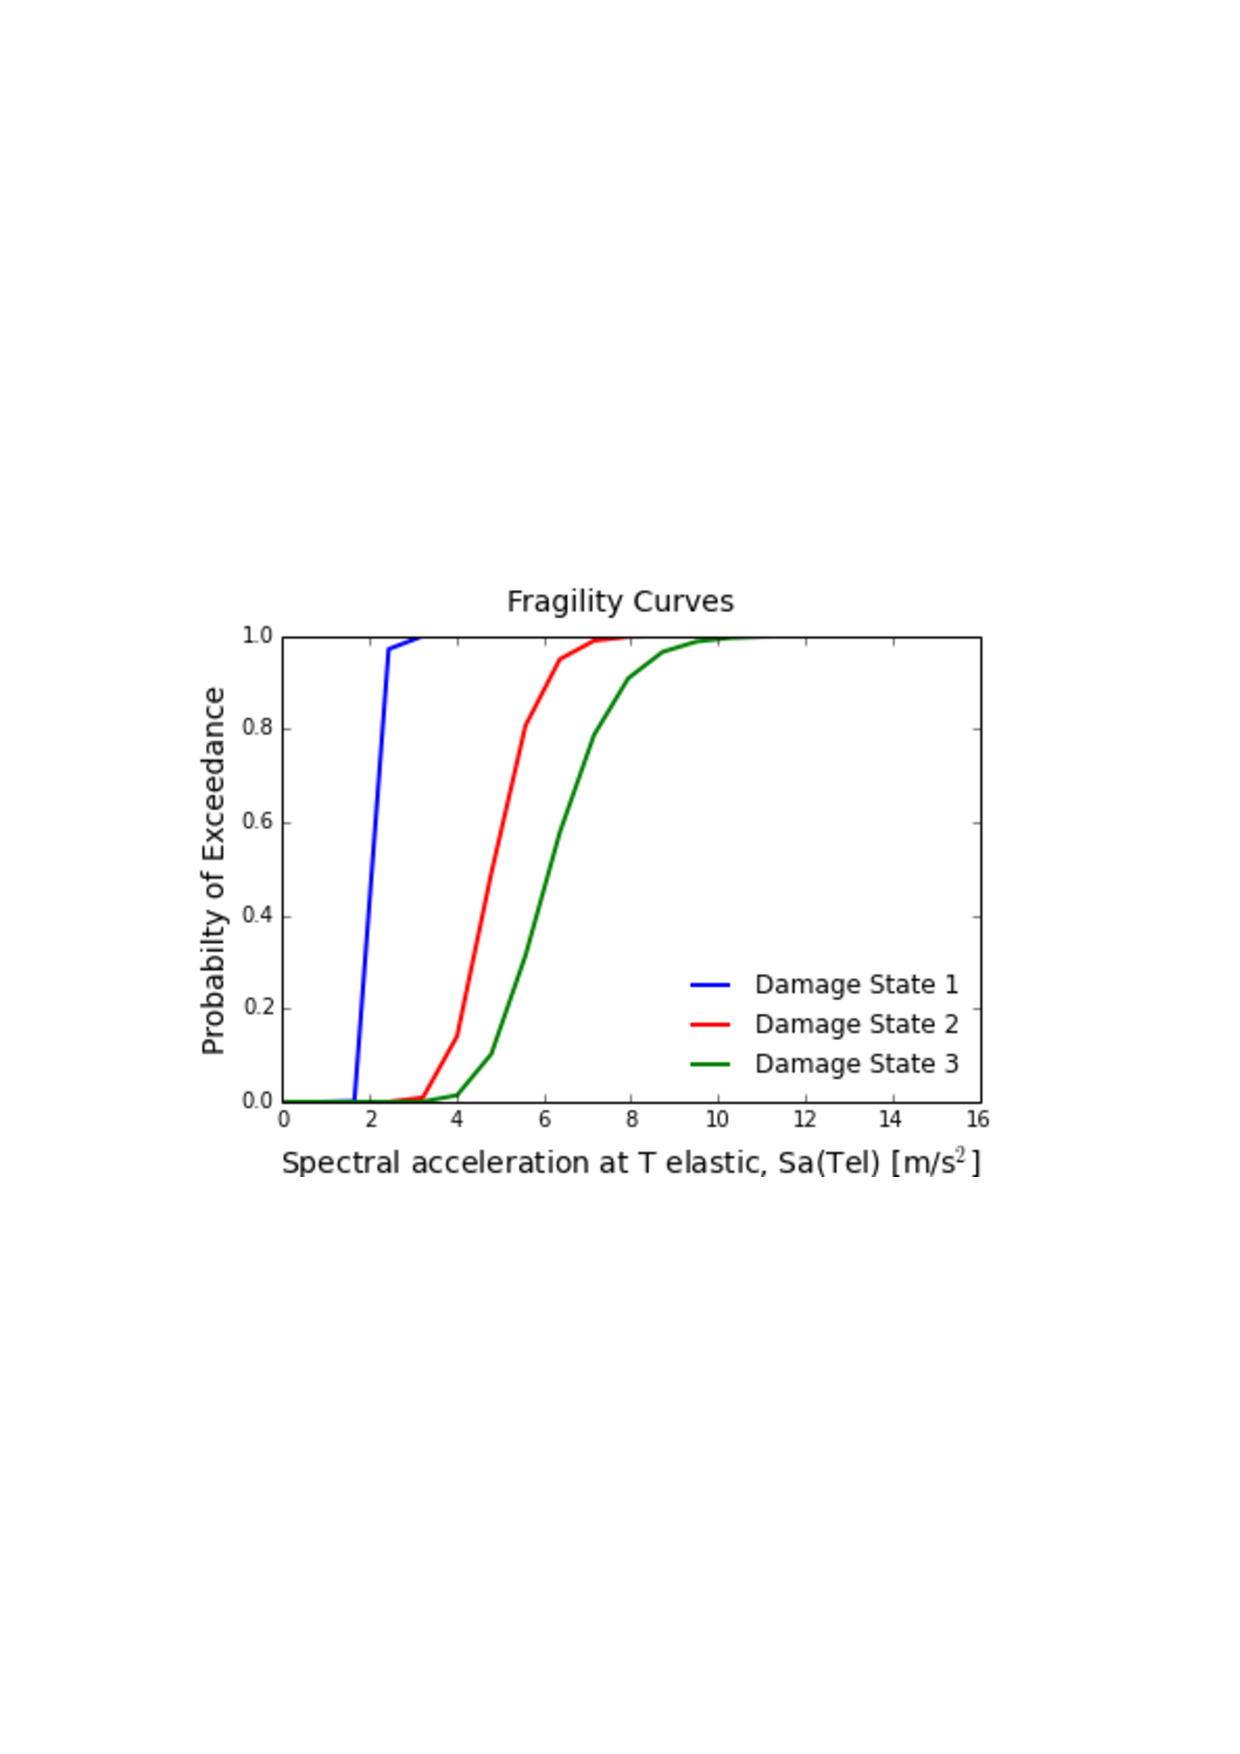
\includegraphics{./figures/IdealisedCurve.pdf}
%\caption{Pushover curve.}
%\label{fig:expPushover}
%\end{figure}

% \begin{pspicture}(0,0)(6cm,6cm)
% 	\psframe[fillstyle=solid,linecolor=white,fillcolor=white]
% 		(0.0cm,6.0cm)(6cm,6cm)	
% 	\rput[l](0cm,6cm){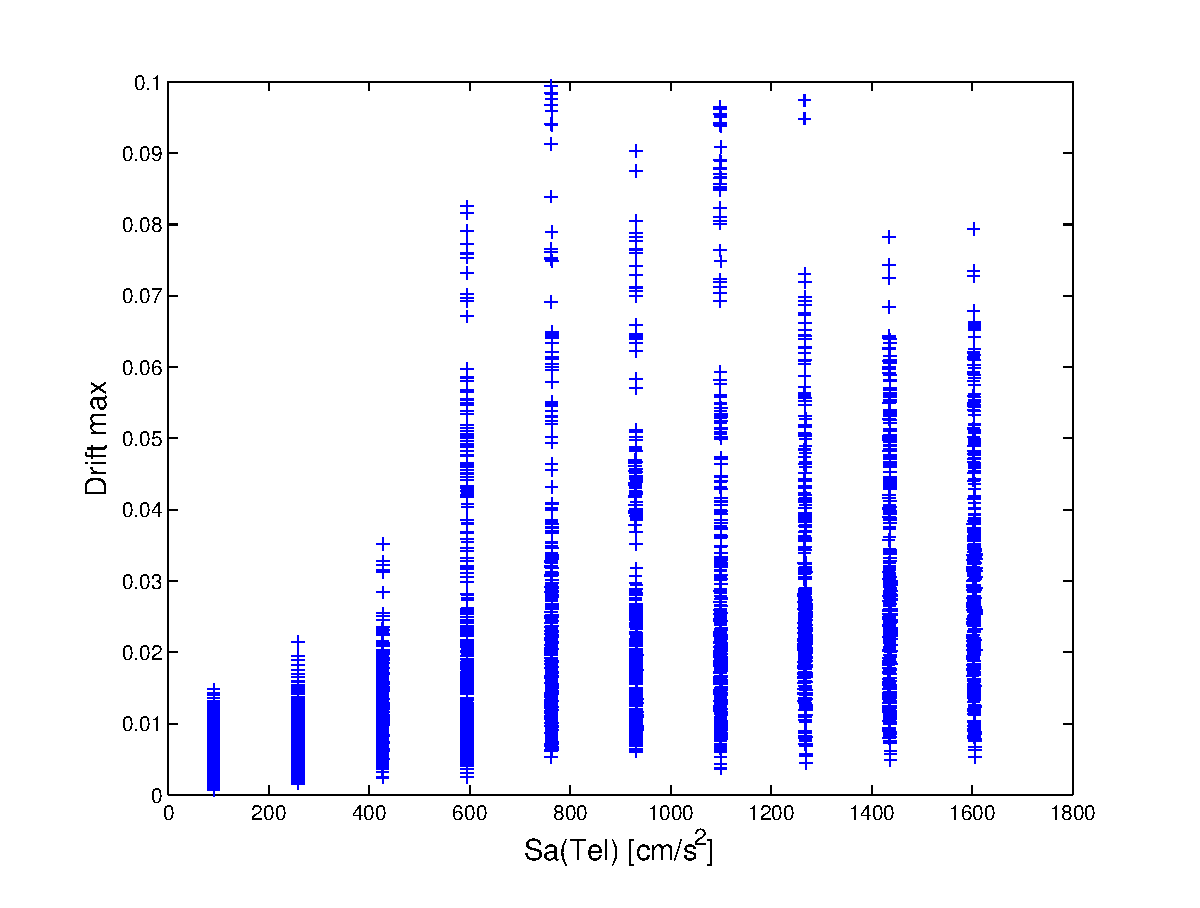
\includegraphics[width=5cm,height=5cm]{./Figures/regression_R3.eps}}
% \end{pspicture}

\begin{figure}[H]
\centering
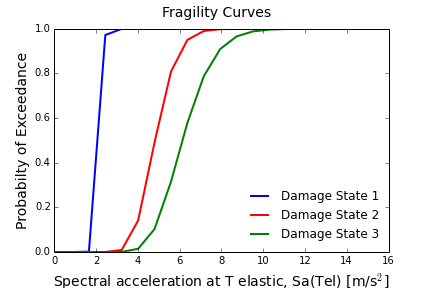
\includegraphics{./figures/PushoverCurve.png}
\caption{Idealised pushover curve.}
\label{fig:expIdealised}
\end{figure}

\item Dynamic parameters of the building: fundamental period of vibration T$_1$ and corresponding modal participation factor $\Gamma_1$.
\item Limit States in terms of roof displacement or inter-storey drift ratio.
\item Consequence function (damage factor for each damage state).
\end{itemize}

\subsubsection{Options}
\label{subsubsec:options}
The type of procedure to be performed and the type of inputs at disposal, are set with the variables \textit{an\_type} and \textit{in\_type} respectively. With the variable \textit{an\_type} the user can choose between:

\begin{Verbatim}[frame=single, commandchars=\\\{\}, samepage=true]
an\_type = 0 #Cr-based procedure (Ruiz-Garcia and Miranda, 2007)
an\_type = 1 #spo2ida-based procedure (Vamvatsikos and Cornell, 2006)
an\_type = 2 #R-$mu$-T-based procedure (Dolsek and Fajfar, 2004)
\end{Verbatim}

With the variable \textit{in\_type} the user can choose between:

\begin{Verbatim}[frame=single, commandchars=\\\{\}, samepage=true]
in\_type = 0 # idealised pushover curve
in\_type = 1 # raw results from a pushover analysis
\end{Verbatim}

The variable \textit{vulnerability} instead gives the opportunity to decide the type of outputs, whether to stop the process at the derivation of the fragility curves, or to go all the way up to the vulnerability curve definition, applying damage-to-loss functions.

\begin{Verbatim}[frame=single, commandchars=\\\{\}, samepage=true]
vuln = 0 # derive fragility curves 
vuln = 1 # derive vulnerability curve
\end{Verbatim}

The variable \textit{g} serves the purpose of defining the units that are being used. A floating number must be assigned to the gravity acceleration, compatible with the units used for the period of vibration and for the displacements (if the period is expressed in seconds and displacements are in meters, then g = 9.81). The variable \textit{iml} is a numpy array that identifies the intensity measure levels for which loss ratios are computed and provided in the vulnerability curve.

\begin{Verbatim}[frame=single, commandchars=\\\{\}, samepage=true]
g = 9.81
iml = np.linspace(0.1,15,100)
\end{Verbatim}

The variable \textit{plotflag} allows or inhibits the displaying of plots. It is a python list composed of 4 integers, each one controlling a different plot: idealised pushover curve, 16\%-50\%-84\% ida curves, fragility curves and vulnerability curve respectively. Each integer can take as value either zero or one, whether the corresponding graph has to be displayed or not:

\begin{Verbatim}[frame=single, commandchars=\\\{\}, samepage=true]
plotflag = [1, 1, 1, 1] # plot all the graphs
plotflag = [0, 0, 0, 0] # do not plot any graph
\end{Verbatim}

The following variables set some of the characteristics of the plots:

\begin{itemize}
\item \textit{linew}: integer for defining lines width.
\item \textit{fontsize}: fontsize used for labels, graphs etc.
\item \textit{units}: list of 3 strings defining displacements, forces and Spectral acceleration units, as ['[kN]', '[m]', '[m/s$^2$]'], to be displayed on the axes of the plots.
\end{itemize}

The following variables are needed for spo2ida-based procedure only:
\begin{itemize}
\item \textit{N}: number of points per segment of IDA curve derived with spo2ida
\item \textit{MC}: number of Monte Carlo simulations to account for uncertainty in damage thresholds
\end{itemize}

The last set of variables is needed for R-$\mu$-T-based procedure only:
\begin{itemize}
\item \textit{Tc}: constant accel-constant velocity corner period of a Newmark-Hall type spectrum. Default value is 0.5.
\textit{Td}: constant velocity-constant displacement corner period of a Newmark-Hall type spectrum. Default value is 1.8.
\end{itemize}

		\subsection{C$_R$-based procedure (Ruiz-Garcia and Miranda, 2007)}
		\label{subsec:nls-ruiz-garcia-miranda}
		The aim of this procedure, proposed by Vamvatsikos (2014), is the estimation of the median spectral acceleration value $\hat{S}_{a,ds}$, that brings the structure to the attainment of a set of damage states \textit{ds}, and the corresponding dispersion beta $\beta_{S_a}$, the parameters needed for the mathematical representation of fragility in equation \ref{eq:fragility-definition}. The aim is achieved making use of the work by Ruiz-Garcia and Miranda (2007), where the inelastic displacement demand is related to the elastic displacement with a simple relationship, and it can thus be easily estimated through a response spectrum analysis and a capacity curve.

The C$_R$-based procedure presented herein is applicable to bilinear elasto-plastic capacity curve only, and it is suitable for single building fragility curve estimation, as described in section \ref{subsubsec:single-building}. However the fragility curves derived for single buildings can be combined in a unique fragility curve, which considers the inter-building uncertainty, as described in the following sections.

\subsubsection{Single Building Fragility and Vulnerability function}
\label{subsubsec:single-building}
This procedure provides a simple relationship between median damage state threshold, expressed in terms of top displacement IS THIS DISPLACEMENT OR DRIFT?? $\hat{d}_{roof, ds}$, at each damage state threshold \textit{ds}, and the corresponding median elastic Spectral displacement value $\hat{S}_{d,ds}(T_1)$.

\begin{equation}
\hat{d}_{roof, ds} = C_R \hat{S}_{d, ds}(T_1) \Gamma_1 \Phi_1
\end{equation}

where $\Gamma_1 \Phi_1$ is the first mode participation factor estimated for the first-mode shape normalised by the roof displacement, and C$_R$ is the inelastic displacement ratio (inelastic over elastic spectral displacement), computed by Ruiz-Garcia and Miranda (2007) for nonlinear SDoF systems having hysteretic behaviour representative of the analysed structure, which is a function of the first-mode period of vibration and the relative lateral strength of the system R. Therefore the median Spectral acceleration at the fundamental period of vibration $\hat{S}_{a,ds}(T_1)$ turns out to be expressed as a function of the roof displacement according to the following equation:

\begin{equation}
\hat{S}_{a,ds}(T_1) = \frac{4 \pi^2}{\hat{C}_R T^2 \Gamma_1 \Phi_1} \hat{d}_{roof, ds}
\label{eq:Sa_RGM}
\end{equation}

Default values of $\hat{C}_R$ parameter estimates are provided by Ruiz-Garcia and Miranda (2007), as result of nonlinear regression analysis of three different measures of central tendency computed from 240 ground motions:

\begin{equation}
\hat{C}_R = 1 + \frac{\hat{R} - 1}{79.12 T_1 ^{1.98}}
\label{eq:Cr_RGM}
\end{equation}

and values for $\hat{R}$ are given as:

\begin{equation}
\hat{R}_{ds} = max(0.425(1 - c + \sqrt{c^2 + 2c(2 \hat{\mu}_{ds} - 1) + 1}),1)
\label{eq:R_RGM}
\end{equation}

where c = 79.12 T$^{1.98}$, and $\hat{\mu}_{ds}$ is the median ductility level at the damage state threshold of interest.

For what concerns $\beta_{S_a}$, the dispersion of $\hat{S}_{a,ds}$, it can be computed either in a simplified way or with a Monte Carlo sampling procedure, only if the dispersion due to uncertainty in the limit state definition $\beta_{\theta c}$ is different from zero.

In the simplified approach the following relationship between $S_a$ and the median EDP damage threshold $\hat{\theta}$ (Cornell, 2002) is used:

\begin{equation}
\hat{\theta} = a S_a^b
\end{equation}

so that $\beta_{S_a}$ can be easily derived from the dispersion of $\theta$ due to record-to-record variability, $\beta_{\theta d}$, as in the following:

\begin{equation}
\beta_{S_a} = \frac{1}{b} \beta_{\theta d}
\label{eq:betaSa_RGM}
\end{equation}

$\beta_{\theta d}$ can be obtained assuming that top drift $d_{roof}$ and $\theta$ are proportional, and they thus share the same dispersion. Moreover the dispersion of $d_{roof}$ is the same as the dispersion of C$_R$, since they are also proportional. Finally $\beta_{\theta d}$ can be computed with the following equation, which represents Ruiz-Garcia and Miranda's (2007) estimate of C$_R$ dispersion:

\begin{equation}
\sigma_{\ln(C_R)} = \sigma_{\ln(d_{roof})} = \beta_{\theta d} =  1.975 [\frac{1}{5.876} + \frac{1}{11.749 (T + 0.1)}] [1- \exp(-0.739 (R - 1))]
\label{eq:beta_eq_RGM}
\end{equation}

Uncertainty in the damage state can also be accounted for combining the dispersion of $\theta$ due to uncertainty in the damage state with the dispersion due to record-to-record variability as in the following equation:

\begin{equation}
\beta_{S_a} = \frac{1}{b} \sqrt{\beta_{\theta d}^2 + \beta_{\theta c}^2}
\label{eq:betaStot_RGM}
\end{equation}

In the Monte Carlo approach first of all three polylines corresponding to the 16$^{th}$, 50$^{th}$ and 84$^{th}$ fractiles of R need to be drawn. This is done by computing $\beta_{\theta d}$ for each median $\hat{\mu}_{ds}$ with eq. \ref{eq:beta_eq_RGM}, and obtaining from this value the 16$^{th}$ and 84$^{th}$ fractiles of $\mu_{ds}$, $\mu_{16\%}$ and $\mu_{84\%}$ according to the following equations:

\begin{equation}
\mu_{ds,16} = \hat{\mu}_{ds} e^{-\beta_{\theta d,ds}}
\end{equation}
\begin{equation}
\mu_{ds,16} = \hat{\mu}_{ds} e^{\beta_{\theta d,ds}}
\end{equation}

The median $\hat{R}_{ds}$ values have been already found from eq. \ref{eq:R_RGM}, and $mu_{16\%}-\hat{R}$, $\hat{\mu}-\hat{R}$ and $\mu_{84\%}-\hat{R}$ curves can be drawn.
Different values of ductility limit state are now sampled from the lognormal distribution with median the median value of the ductility limit state, and dispersion the input $\beta_{\theta c}$.
For each of these ductilities the corresponding $\hat{R}$,$R_{16\%}$, and $R_{84\%}$ values are found interpolating the aforementioned curves, and converted into $\hat{S}_{a,ds}$ and $\beta_{\theta d}$ according to the following equations:

\begin{equation}
\hat{S}_{a,ds} = \hat{R}(\mu_{ds}) S_{ay}
\label{eq:SaR}
\end{equation}
\begin{equation}
\beta_{R(\mu)} = \frac{\ln R(\mu)_{84\%} - \ln R(\mu)_{16\%}}{2}
\label{eq:betaR}
\end{equation} 

where
\begin{equation}
S_{ay} = \frac{4 \pi^2 d_{roof,y}}{T_1^2 g \Gamma_1}
\label{eq:Say}
\end{equation}

N random S$_a$ for each of the N sampled ductility limit states are computed using $\hat{S}_{a,ds}$ and $\beta_{\theta d}$, and their median and the dispersion are estimated. These parameters constitute the median $\hat{S}_{a,ds}$ and the total dispersion $\beta_{S_a}$ for the considered damage state. The procedure is repeated for each damage state.

To derive a discrete vulnerability function at certain intensity measure levels, the input damage-to-loss factors are applied to the probability of occurance of each damage state, extracted from the probability of exceedance of each damage state described by the fragility function. A value of loss ratio is thus defined for the vector of selected intensity measure levels.

\subsubsection{Multiple-Building Fragility and Vulnerability function}
\label{subsubsec:multiple-buildings}
If multiple buildings have been input to derive fragility function for a class of buildings all $\hat{S}_{a, blg}$ and $\beta_{S_a, blg}$ are combined in a single lognormal curve. A minimum of 5 buildings should be considered to obtain reliable results for the class. 
A new issue arises when multiple buildings are considered: the S$_a$ at the fundamental period of each building should be converted to a common intensity measure, to be able to combine the different fragility functions. A common intensity measure is selected to be S$_a$ at the period T$_{av}$, which is a weighted average of the individual buildings fundamental period T$_1$. Then each individual fragility needs to be expressed in terms of the common S$_a$(T$_{av}$), using a spectrum. FEMA P-695 far field set of 44 accelerograms (22 records for the two directions) was used to derive a mean uniform hazard spectrum, and the ratio between the S$_a$ at different periods is used to scale the fragility functions. It can be noted that the actual values of the spectrum are not important, but just the spectral shape. 
The median $\hat{S}_a$ is converted to the mean $\mu_{ln(S_a)}$ of the corresponding normal distribution ($\mu_{ln(S_a)} = ln(\hat{S}_a)$) and, simply scaled to the common intensity measure as follows:

\begin{equation}
\mu_{ln(S_a), blg} = \mu_{ln(S_a), blg} S(T_{av})/ S(T_{1, blg})
\end{equation}
\begin{equation}
\beta_{S_a, blg} = \beta_{S_a, blg} S(T_{av})/ S(T_{1, blg})
\label{eq:Sa(Tav)}
\end{equation}

Finally the parameters of the single lognormal curve for the class of buildings, mean and dispersion, can be computed as the weighted mean of the single means and the weighted SRSS of the inter-building and intra-building standard deviation, the standard deviation of the single means and the single dispersions respectively, as shown in the following equations:

\begin{equation}
\mu_{ln(S_a), tot} = \sum_{i=0}^{n.blg} w_{blg-i} \mu_{ln(S_a), blg-i}
\label{eq:combination-lognormals-mu}
\end{equation}
\begin{equation}
\beta_{S_a, tot} = \sqrt{ \sum_{i=0}^{n.blg} w_{blg-i} ((\mu_{ln(S_a), blg-i}-\mu_{ln(S_a), tot})^2+ \beta_{S_a, blg-i}^2})
\label{eq:combination-lognormals-sigma}
\end{equation}

The mean $\mu_{ln(S_a)}$ and total dispersion $\beta_{S_a}$ of the fragility function of the class are converted to logarithmic mean $\mu_{S_a}$ and logarithmic covariance $cov_{S_a}$ (standard deviation $\sigma_{S_a}$ over $\mu_{S_a}$), according to the following equations:

\begin{equation}
\hat{S}_a = e^{\mu_{ln(S_a)}}
\end{equation}
\begin{equation}
\mu_{S_a} = \hat{S}_a e^{\frac{\beta_{S_a}^2}{2}}
\label{eq:median-to-mean}
\end{equation}
\begin{equation}
\sigma_{S_a} = \sqrt[2]{(\beta_{S_a}^2-1) e^{2\ln{ \hat{S}_a}+\beta_{S_a}^2}}
\label{eq:dispersion-to-standard}
\end{equation}
\begin{equation}
cov_{S_a} = \frac{\sigma_{S_a}}{\mu_{S_a} }
\end{equation}

A single vulnerability function can be also obtained, from the single building vulnerability functions. The input damage-to-loss function is applied to the fragility function derived for each building. For the selected intensity measure levels a value of loss ratio $LR_{blg}$ is thus defined for each building. A discrete vulnerability function for the entire class of buildings is represented at each iml by a mean LR, $\mu_{LR,tot}$, equal tot the weighted $LR_{blg}$, and a standard deviation, $\sigma_{LR, tot}$, equal to the weighted standard deviation of all the computed $LR_{blg}$. The $\sigma_{LR, tot}$ of the fragility function of the class is converted to covariance $cov_{LR}$ (standard deviation $\sigma_{LR, tot}$ over $\mu_{LR, tot}$).

\subsubsection{Inputs}
\label{subsubsec:InputCr}
The inputs must be formatted as comma-separated value files (.csv), and saved in the folder \textit{input}, contained in the NSP directory. If any other environment different from Windows is used make sure that the "comma separated values Windows" is selected as saving option when creating the input files. 

If multiple buildings want to be analysed to consider the inter-building uncertainty the parameters relative to each building should be added as additional lines in the input tables, as shown in the examples below, otherwise a single line must be input.

If the user has already at disposal an idealised elasto-plastic pushover curve for each building, that is to say that the variable \textit{in\_type} has been set to 0, the following data need to be provided in the corresponding csv files:

\begin{enumerate}
\item First period of vibration T$_1$, corresponding modal participation factor $\Gamma_1$, normalised with respect to the roof displacement, and weight for the combination of different buildings, input in \textit{building\_parameters.csv}, as in the example below:
	\begin{table}[!htbp]
	\centering
	\begin{tabular}{|c|c|c|c|} \hline
	\textbf{n.building} & \textbf{T$_1$} & \textbf{$\Gamma_1$} & \textbf{weights}\\ \hline
	1 & 0.32 & 1.23 & 0.2\\ \hline
	2 & 0.40 & 1.25 & 0.3\\ \hline
	... & ... & ... & ... \\ \hline
	\end{tabular}
	\end{table}
	
\item Roof displacement at each limit state LS and corresponding dispersion $\beta_{\theta c}$ input in \textit{displacement\_profile.csv}, as shown in the example below. If dispersion is unknown, $\beta_{\theta c}$ can be set equal to zero at each LS.
	\begin{table}[!htbp]
	\centering
	\begin{tabular}{|c|c|c|c|} \hline
	\textbf{n.building} & \textbf{LS$_1$} &	\textbf{LS$_2$} &	\textbf{LS$_3$} \\ \hline
	1 & 0.066 & 0.169 & 0.23\\ \hline
	$\beta_{\theta d, 1}$ & 0.1 & 0.3 & 0.4\\ \hline
	2 & 0.08 & 0.172 & 0.25\\ \hline
	$\beta_{\theta d, 2}$ & 0.1 & 0.3 & 0.4\\ \hline	
	\end{tabular}
	\end{table}
	
\item Idealised pushover curve, input in \textit{idealised\_curve.csv} as shown below. The only required parameters are the yielding displacement $d_y$, the ultimate displacement $d_u$ and the yielding force F$_y$.

\begin{table}[!htbp]
\centering
\begin{tabular}{|c|c|c|c|} \hline
\textbf{n.building} & \textbf{d$_y$} & \textbf{d$_u$} & \textbf{F$_y$} \\ \hline
1 & 0.09	& 0.3	 & 523\\ \hline
2 & 0.12	& 0.35	 & 400\\ \hline
... & ...	& ... & ...\\ \hline
\end{tabular}
\end{table}

\item Consequence model (loss ratio per each damage state) consistent with the defined set of damage states, input in \textit{consequence.csv}, as in the example below. A single consequence model can be input. This input is needed only if the variable \textit{vuln} has been set to 1.	
	\begin{table}[!htbp]
	\centering
	\begin{tabular}{|c|c|c|} \hline
	\textbf{DS$_1$} & \textbf{DS$_2$} & \textbf{DS$_3$} \\ \hline
	0.2	& 0.5	 & 1\\ \hline
	\end{tabular}
	\end{table}
	
\end{enumerate}

If the idealised curve are not available, \textit{in\_type} = 0 can be selected and the displacements vs base shear at each time step results from a pushover analysis can be input instead. The following data need to be provided in the corresponding csv files:

\begin{enumerate}
\item T$_1$ and corresponding $\Gamma_1$, weight for the combination of different buildings, number of storeys and height of each storey, input in \textit{building\_parameters.csv}, as in the example below:
	\begin{table}[!htbp]
	\centering
	\begin{tabular}{|c|c|c|c|c|c|c|c|c|} \hline
	\textbf{n.building} & \textbf{T$_1$} & \textbf{$\Gamma_1$} & \textbf{weights} & \textbf{n.Storey} & \textbf{H$_1$} & \textbf{H$_2$} & ... & \textbf{H$_n$} \\ \hline
	1 & 0.32 & 1.23 & 0.2 & 4 & 3 & 3 & ... & 3 \\ \hline
	2 & 0.40 & 1.25 & 0.3 & 4 & 4 & 2.7 & ... & 2.7 \\ \hline
	... & ... & ... & ... & ... & ... & ... & ... & ... \\ \hline
	\end{tabular}
	\end{table}
	
\item Displacements at each storey, at each incremental step of the pushover analysis, input in \textit{displacements\_pushover.csv}, as in the example below: 
	\begin{table}[!htbp]
	\centering
	\begin{tabular}{|c|c|c|c|c|c|c|} \hline
	\textbf{n.building} & \textbf{n.Storey} & \textbf{Step1} & \textbf{Step 2} & \textbf{Storey 3} & ... & \textbf{Step n}\\ \hline
	1 &	1 & 0.0001 &	0.0005 &	0.001 & ... & 0.01\\ \hline
	   &	2 & 0.0003 &	0.0010 &	0.002 & ... & 0.02\\ \hline
	   &	3 & 0.0004 &	0.0016 &	0.003 & ... & 0.03\\ \hline
	   &	4 & 0.0006 &	0.0021 &	0.004 & ... & 0.04\\ \hline
	2 &	1 & 0.0001 &	0.0005 &	0.001 & ... & 0.01\\ \hline
	   &	2 & 0.0005 &	0.0012 &	0.002 & ... & 0.03\\ \hline
	   &	... & ... &	... &	... & ... & ...\\ \hline
	\end{tabular}
	\end{table}
	
\item Base shear at each incremental step of the pushover analysis input in \textit{reactions\_pushover.csv}, as in the example below:
	\begin{table}[!htbp]
	\centering
	\begin{tabular}{|c|c|c|c|c|c|} \hline
	\textbf{n.building} &	\textbf{Step1} & \textbf{Step 2} & \textbf{Storey 3} & ... & \textbf{Step n} \\ \hline
	1 & 0.35 & 0.69 & 1.04 & ... & 29.12\\ \hline
	2 & 0.45 & 0.78 & 2.05 & ... & 40.00\\ \hline
	... & ... & ... & ... & ... & ...\\ \hline
	\end{tabular}
	\end{table}
	
\item Drift limit state and corresponding dispersion $\beta_{\theta c}$ input in \textit{limits.csv}. If dispersion is unknown, $\beta_{\theta c}$ can be set equal to zero at each limit state.
	\begin{table}[!htbp]
	\centering
	\begin{tabular}{|c|c|c|c|} \hline
	\textbf{n.building} & \textbf{LS$_1$} &	\textbf{LS$_2$} &	\textbf{LS$_3$} \\ \hline
	1 & 0.01 &	0.025 & 0.0337\\ \hline
	$\beta_{\theta d, 1}$ &	0.1 & 0.2 & 0.25\\ \hline
	2 & 0.014 &	0.030 & 0.0430\\ \hline
	$\beta_{\theta d, 2}$ &	0.1 & 0.2 & 0.25\\ \hline
	\end{tabular}
	\end{table}

\item Consequence model (loss ratio per each damage state) consistent with the defined set of damage states, input in \textit{consequence.csv}, as in the example below. A single consequence model can be input. This input is needed only if the variable \textit{vuln} has been set to 1.
	\begin{table}[!htbp]
	\centering
	\begin{tabular}{|c|c|c|} \hline
	\textbf{DS$_1$} & \textbf{DS$_2$} & \textbf{DS$_3$} \\ \hline
	0.2	& 0.5	 & 1\\ \hline
	\end{tabular}
	\end{table}
	
\end{enumerate}

\subsubsection{Calculation Steps}
The overall workflow of C$_R$-based procedure is summarised in this section. The option \textit{an\_type} must be set equal to 0 and the option \textit{in\_type} according to the input at disposal. The corresponding inputs should follow the requirements described in section \ref{subsubsec:InputCr}. At this point the code proceeds with the following steps:

\begin{enumerate}
\item
\begin{enumerate}
\item If \textit{in\_type} = 0 roof displacement at limit states and idealised pushover are extracted from \textit{displacement\_profile.csv} and \textit{idealised\_curve.csv} respectively.
\item If \textit{in\_type} = 1 results from pushover analysis are extracted from \textit{displacements\_pushover.csv} and \textit{reactions\_pushover.csv}, and drift limit states from \textit{limits.csv}. The idealised 	pushover curve is then derived in the \textit{idealisation} function, where the idealisation process is conducted according to FEMA-440. The elastic stiffness is defined as the 	tangent stiffness passing through the point of the pushover curve where 60\% of the maximum base shear is reached, and the perfectly plastic branch is set at an height equal to 	the maximum base shear. The yielding point is found as the interception between the elastic and the plastic branch.
\end{enumerate}

\item The csv input files are parsed with the function \textit{read\_data} according to the defined options. The parameters essential to the analysis are return together with a graphical visualisation of the inputs if the variable \textit{plotflag}[0] is equal to 1.

\item The parameters extracted are used in the \textit{simplified\_bilinear} function, within the \textit{fragility\_process} function, to derive ductility levels $\mu_{ds}$, median spectral acceleration $\hat{S}_{a,ds}$ and the total dispersion $\beta_{S_a}$ at each limit state through the following steps:
\begin{itemize}
\item The idealised MDoF system is transformed into an equivalent SDoF system, using $\Gamma_1$.
\item Ductility levels $\mu_{ds}$ corresponding to each damage threshold, are defined.
\item R and C$_R$ are computed, using eq. \ref{eq:R_RGM} and \ref{eq:Cr_RGM} respectively.
\item $\hat{S}_{a,ds}$ and the corresponding dispersion  $\beta_{\theta d}$ are computed using eq. \ref{eq:Sa_RGM} and \ref{eq:betaSa_RGM} respectively.
\item If dispersion due to uncertainty in the limit state $\beta_{\theta c}$ is different from zero different ductility limit states are sampled for each median ductility level $\mu_{ds}$ and corresponding values of $\hat{S}_{a,ds}$ and $\beta_{S_{a, d}}$ are computed, as described in section \ref{subsubsec:single-building}, but not yet combined together..
\end{itemize}

\item All $\hat{S}_{a, ds}(T_1)$ are converted to mean $\mu_{ln(S_{a, ds})}(T_1)$ and then to the intensity measure in common with the rest of the buildings, $\mu_{ln(S_{a, ds}(T_{av}))}$, according to eq. \ref{eq:Sa(Tav)}.

\item Step 3 and 4. are repeated for the number of input buildings.

\item
\begin{enumerate}
\item If \textit{vuln} = 0: All $\hat{S}_{a,ds}$ and $\beta_{S_{a, d}}$ from all the buildings and all the sampled ductility limit states are combined in a single lognormal curve, as described in section \ref{subsubsec:single-building-spo2ida}. 
Mean $\mu_{ln(S_{a})}$ and total dispersion $\beta_{S_a}$ are then converted to logarithmic mean $\mu_{S_a}$ and logarithmic covariance $cov_{S_a}$, according to equations \ref{eq:median-to-mean} and \ref{eq:dispersion-to-standard} respectively.
Fragility curves for the class of buildings are displayed if the variable \textit{plotflag}[2] = 1, and logarithmic $\mu_{S_a}$ and $cov_{S_a}$ are exported in the \textit{outputs} folder.
\item If \textit{vuln} =1:  
For the intensity measure levels defined in the variable \textit{iml} a value of loss ratio $\mu_{LR, iml, blg}$ is defined for each building and a standard deviation $\sigma_{LR, iml, blg}$, if dispersion due to uncertainty in the limit state $\beta_{\theta c}$ is different from zero. They are finally combined in a single mean and standard deviationas described in section \ref{subsubsec:multiple-building-spo2ida}. Vulnerability curve for the class of buildings is displayed if the variable \textit{plotflag}[3] = 1, and $\mu_{LR}$ and $cov_{LR}$ at each iml are exported in the \textit{outputs} folder.
\end{enumerate}
\end{enumerate}


		\subsection{spo2ida-based procedure (Vamvatsikos and Cornell, 2006)}
		\label{subsec:nls-spo2ida}
		The aim of this procedure is the estimation of the median spectral acceleration value $\hat{S}_{a,ds}$, that brings the structure to the attainment of a set of damage states ds, and the corresponding dispersion beta $\beta_{S_a}$, the parameters needed for the mathematical representation of fragility in equation \ref{eq:fragility-definition}. The aim is achieved making use of the tool spo2ida (Vamvatsikos and Cornell, 2006), where static pushover curves are converted into 16\%, 50\% and 84\% IDA curves, using empirical relationships from a large database of incremental dynamic analysis results, as shown in Figure~\ref{fig:spo2ida}.

\begin{figure}[H]
\centering
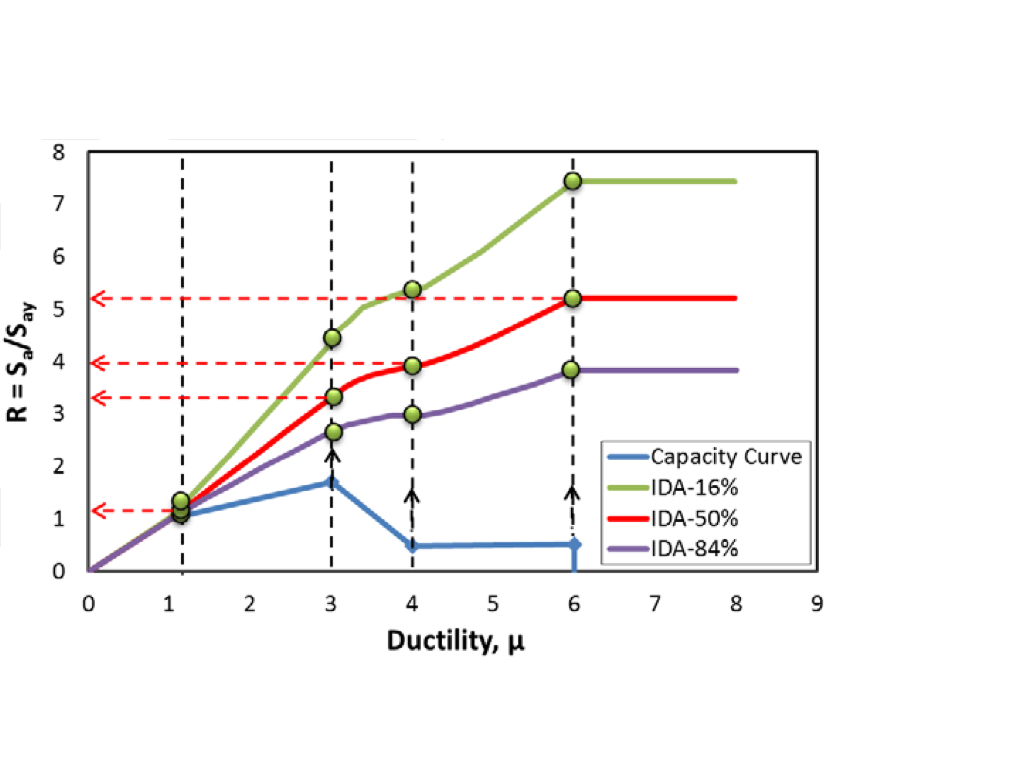
\includegraphics[width=12cm,height=8cm]{./figures/spo2ida.jpg}
\caption{spo2ida tool: IDA curves derived from Pushover curve.}
\label{fig:spo2ida}
\end{figure}

The spo2ida-based procedure presented herein is applicable to any kind of multi-linear capacity curve, and it is suitable for single building fragility curve estimation, as described in section \ref{subsubsec:single-building-spo2ida}. However the fragility curves derived for single buildings can be combined in a unique fragility curve, which considers the inter-building uncertainty, as described in section \ref{subsubsec:multiple-building-spo2ida}.

\subsubsection{Single-building Fragility and Vulnerability function}
\label{subsubsec:single-building-spo2ida}
Given the idealised capacity curve the spo2ida tool uses an implicit R-$\mu$-T relation to correlate nonlinear displacement, expressed in terms of ductility $\mu$ to the corresponding medians capacity in terms of the parameters R. R is the lateral strength ratio, defined as the ratio between the spectral spectral acceleration S$_a$ and the yielding capacity of the system S$_{ay}$. 

Each branch of the capacity curve, hardening, softening and residual plateau, is converted to a corresponding branch of the three ida curves, using the R-$\mu$-T relation, which is a function of the hardening stiffness, the softening stiffness and the residual force. These parameters are derived from the idealised pushover capacity expressed in $\mu$-R terms, as well as the ductility levels at the onset of each branch. If some of the branches of the pushover curve are missing because of the seismic behaviour of the system, spo2ida can equally work with bilinear, trilinear and quadrilinear idealisations.

The result of the spo2ida routine is thus a list of ductility levels and corresponding R values at 50\%, 16\% and 84\% percentiles. The distribution of R values at each ductility level, due to the record-to-record variability, is assumed to be lognormal and it can be easily converted to the dispersion of the lognormal distribution with the following equation:

\begin{equation}
\beta_{R(\mu)} = \frac{\ln R(\mu)_{84\%} - \ln R(\mu)_{16\%}}{2}
\label{eq:betaR}
\end{equation} 

$\beta_{R(\mu)}$ represents also the record-to-record variability of S$_a$ at different ductility levels $\beta_{S_a, d}$. Median R and its dispersion at ductility levels corresponding to the damage thresholds can thus be determined, and $\hat{S}_{a,ds}$ can be easily extracted simply multiplying $R_{50\%}(\mu_{ds})$ by the yielding capacity of the system $S_{ay}$, as shown in the following equation:

\begin{equation}
\hat{S}_{a,ds} = R_{50\%}(\mu_{ds}) S_{ay}
\label{eq:SaR}
\end{equation}
\begin{equation}
S_{ay} = \frac{4 \pi^2 \delta_{roof,y}}{g \Gamma_1 T_1^1}
\end{equation}

Since $\hat{R}$ and $\hat{S}_{a}$ are proportional they share the same dispersion.

If dispersion due to uncertainty in the limit state definition $\beta_{\theta c}$ is different from zero it can not be combined directly with the record-to-record dispersion, but a Monte Carlo sampling of the limit state needs to be performed instead. Different values of ductility limit state are sampled from the  lognormal distribution with median the median value of the ductility limit state, and dispersion the input $\beta_{\theta c}$. For each of these ductilities the corresponding R$_{16\%}$-R$_{50\%}$-R$_{84\%}$ are found and converted into $\hat{S}_{a,ds}$ and $\beta_{\theta d}$ according to equation \ref{eq:SaR} and \ref{eq:betaR}. N random S$_a$ corresponding to the N sampled ductility limit states are computed, and their median and the dispersion are estimated. These parameters constitute the median $\hat{S}_{a,ds}$ and the total dispersion $\beta_{S_a}$ for the considered damage state. The procedure is repeated for each damage state.

To derive a discrete vulnerability function at certain intensity measure levels, the input damage-to-loss factors are applied to the probability of occurance of each damage state, extracted from the probability of exceedance of each damage state described by the set of fragility curves. 

If dispersion due to uncertainty in the limit state is different from zero a vulnerability function is derived for the N sets of sampled ductility limit states. It results in N loss ratios for each defined intensity measure levels. Finally a lognormal distribution of the loss ratios is assumed at each iml and the vulnerability curve is defined at each iml by the mean and the standard deviation of all the computed loss ratios.

\subsubsection{Multiple-Building Fragility and Vulnerability function}
\label{subsubsec:multiple-building-spo2ida}
If multiple buildings have been input to derive a set of fragility curves for a class of buildings all $\hat{S}_{a,blg}$ and $\beta_{S_a,blg}$ are combined in a single lognormal curve for each damage state. A minimum of 5 buildings should be considered to obtain reliable results for the class. The procedure to get $\mu_{S_a,tot}$ and $cov_{S_a,tot}$ for the class of building is the same described in section \ref{subsubsec:multiple-buildings}, but the $\hat{S}_{a,blg}$ and $\beta_{S_a,blg}$ are those derived from each sampled set of ductility limit state.

A single vulnerability curve can also be obtained, from the single building vulnerability curves. If no dispersion in the limit state is defined, the method is the same described in section \ref{subsubsec:multiple-buildings}. Otherwise a vulnerability curve is derived for each building as explained in section \ref{subsub:single-building-spo2ida}, considering the sampled set of ductility limit states, that is to say that the mean loss ratio and its standard deviation at each iml, $\mu_{LR,iml,blg}$ and $\sigma_{LR,iml,blg}$ respectively, are found for each building.
Finally the mean loss ratio and its standard deviation, $\mu_{LR,iml}$ and $\sigma_{LR,iml}$, are found for the entire class of buildings as the weighted mean of the single $\mu_{LR,iml,blg}$ and the weighted SRSS of the inter-building and intra-building standard deviation, the standard deviation of the single means $\mu_{LR,iml,blg}$ and the single dispersions $\sigma_{LR,iml,blg}$ respectively, as described in eq \ref{eq:combination-lognormals-sigma}, substituting loss ratio to spectral acceleration.

\subsubsection{Inputs}
\label{subsubsec:InputSpo2ida}
The inputs must be formatted as comma-separated value files (.csv), and saved in the folder \textit{input}, contained in the NSP directory. If any other environment different from Windows is used make sure that the "comma separated values Windows" is selected as saving option when creating the input files. 

If multiple buildings want to be analysed to consider the inter-building uncertainty the parameters relative to each building should be added as additional lines in the tables, as shown in the examples below, otherwise a single line must be input.

If the user has already at disposal an idealised multilinear pushover curve for each building, that is to say that the variable \textit{in\_type} has been set to 0, the following data need to be provided in the corresponding csv files:

\begin{enumerate}
\item First period of vibration $T_1$, corresponding modal participation factor $\Gamma_1$, normalised with respect to the roof displacement, and weight for the combination of different buildings, input in \textit{building\_parameters.csv}, as in section \ref{subsubsec:InputCr}, input n. 1.
	
\item Top displacement at each damage state threshold and corresponding dispersion $\beta_{\theta c}$ input in \textit{displacement\_profile.csv}, as in section \ref{subsec:InputCr}, input n. 2. 
	
\item Idealised pushover curve, input in \textit{idealised\_curve.csv} as shown below. The parameters needed to describe the idealised pushover curve are: yielding displacement d$_y$, displacement at the onset of degradation d$_s$, displacement at the onset of residual force d$_{min}$, ultimate displacement d$_u$, maximum force F$_{max}$, residual force F$_{min}$. These parameters are represented in Figure~\ref{fig:quadrilinear}.

\begin{figure}[H]
\centering
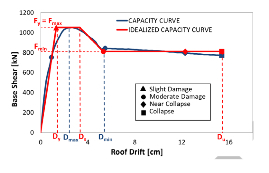
\includegraphics[width=12cm,height=8cm]{./figures/quadrilinear.jpg}
\caption{Idealisation of capacity curve using multilinear elasto-plastic form.}
\label{fig:quadrilinear}
\end{figure}

\begin{table}[H]
\centering
\begin{tabular}{|c|c|c|c|c|c|c|} \hline
\textbf{n.building} & \textbf{d$_y$} & \textbf{d$_s$} & \textbf{d$_{min}$} & \textbf{d$_u$} & \textbf{F$_{max}$} & \textbf{F$_{min}$} \\ \hline
1 & 0.09	& 0.3	& a & b & 523 & 430\\ \hline
2 & 0.12	& 0.35	 & a & b & 400 & 305\\ \hline	
\end{tabular}
\end{table}

\item Consequence model (loss ratio per each damage state) consistent with the defined set of damage states, input in \textit{consequence.csv}, as in section \ref{subsubsec:InputCr}, input n. 5.
	
\end{enumerate}

If these data are not available, \textit{in\_type} = 0 can be selected and the "raw" results from a pushover analysis can be input instead. The same data as in section \ref{subsubsec:InputCr} for \textit{in\_type} = 0 can be input.

\subsubsection{Calculation Steps}
The overall workflow of spo2ida-based procedure is summarised in this section. The option \textit{an\_type} must be set equal to 1 and the option \textit{in\_type} according to the input at disposal. The corresponding inputs should follow the requirements described in section \ref{subsec:InputSpo2ida}. At this point the code proceeds with the following steps:

\begin{enumerate}
\item 
\begin{enumerate}
\item If \textit{in\_type} = 0, the roof displacement at each limit state and the idealised pushover curve parameters are extracted from \textit{displacement\_profile.csv} and \textit{idealised\_curve.csv} respectively.

\item If \textit{in\_type} = 1 the results from a pushover analysis are extracted from \textit{displacements\_pushover.csv} and \textit{reactions\_pushover.csv} and drift limit states from {limits.csv}. The idealised pushover curve is then derived in the \textit{idealisation} function, where the idealisation process is conducted according to the Gem Analytical Vulnerability Guidelines.	\end{enumerate}

\item The parameters extracted are used to derive ductility levels $\mu_{ds}$, median spectral acceleration $\hat{S}_{a,ds}$ and the total dispersion $\beta_{S_a}$ at each damage threshold through the following steps:
\begin{itemize}
\item The idealised MDoF system is transformed into an equivalent SDoF system, using $\Gamma_1$, and SDoF capacity curve is  expressed in terms of $\mu$-R.

\item The variables for spo2ida tool are extracted from the capacity curve and they are used as input to get the 16\%-50\%-84\% ida curves.

\item The ductility levels $\mu_{ds}$ corresponding to each damage threshold are defined, and the corresponding R$_{16\%}$-R$_{50\%}$-R$_{84\%}$ are found in ida outputs.

\item $\hat{S}_{a,ds}$ and the corresponding dispersion $\beta_{S_{a, d}}$ are computed using eq.~\ref{eq:SaR} and eq.~\ref{eq:betaR}, respectively.

\item If dispersion due to uncertainty in the limit state $\beta_{\theta c}$ is different from zero different ductility limit states are sampled for each median ductility level $\mu_{ds}$ and corresponding values of $\hat{S}_{a,ds}$ and $\beta_{S_{a, d}}$ are computed, as described in section \ref{subsubsec:single-building-spo2ida}, but not yet combined together.

\end{itemize}

\item All $\hat{S}_{a, ds}(T_1)$ are converted to mean $\mu_{ln(S_{a, ds})}(T_1)$ and then to the intensity measure in common with the rest of the buildings, $\mu_{ln(S_{a, ds}(T_{av}))}$, according to eq. \ref{eq:Sa(Tav)}.

\item Step 2. and 3. are repeated for the number of input buildings.

\item
\begin{enumerate}

\item If vulnerability = 0: All $\hat{S}_{a,ds}$ and $\beta_{S_{a, d}}$ from all the buildings and all the sampled ductility limit states are combined in a single lognormal curve, as described in section \ref{subsubsec:single-building-spo2ida}. 
Mean $\mu_{ln(S_{a})}$ and total dispersion $\beta_{S_a}$ are then converted to logarithmic mean $\mu_{S_a}$ and logarithmic covariance $cov_{S_a}$, according to equations \ref{eq:median-to-mean} and \ref{eq:dispersion-to-standard} respectively.
Fragility curves for the class of buildings are displayed if the variable \textit{plotflag}[2] = 1, and logarithmic $\mu_{S_a}$ and $cov_{S_a}$ are exported in the \textit{outputs} folder.
\item If vulnerability =1:  
For the intensity measure levels defined in the variable \textit{iml} a value of loss ratio $\mu_{LR, iml, blg}$ is defined for each building and a standard deviation $\sigma_{LR, iml, blg}$, if dispersion due to uncertainty in the limit state $\beta_{\theta c}$ is different from zero. They are finally combined in a single mean and standard deviationas described in section \ref{subsubsec:multiple-building-spo2ida}. Vulnerability curve for the class of buildings is displayed if the variable \textit{plotflag}[3] = 1, and $\mu_{LR}$ and $cov_{LR}$ at each iml are exported in the \textit{outputs} folder.
\end{enumerate}

\end{enumerate}

		\subsection{$R-mu-T$-based procedure (Dolsek and Fajfar, 2004)}
		\label{subsec:nls-dolsek-fajfar}
		The aim of this procedure is the estimation of the median spectral acceleration value $\hat{S}_a$, that brings the structure to the attainment of a set of damage states, and the corresponding dispersion beta $\beta_{S_a}$, the parameters needed for the mathematical representation of fragility in equation \ref{eq:fragility-definition}. The aim is achieved making use of a R-$\mu$-T relationship, between the reduction factor R, the ductility $\mu$ and period T, which is based on the work of Dolsek and Fajfar (2004). The R-$\mu$-T-based procedure presented herein is applicable to any kind of multi-linear capacity curve, and it is suitable for single building fragility curve estimation, as described in section \ref{subsubsec:single-building-DF}. However the fragility curves derived for single buildings can be combined in a unique fragility curve, which considers the inter-building uncertainty, as described in section \ref{subsubsec:multiple-building-DF}.

\subsubsection{Single Building Fragility and Vulnerability function}
\label{subsubsec:single-building-DF}
The spectral value at each damage state threshold \textit{ds} $\hat{S}_{a,ds}$ is found from the roof displacement limit state for that \textit{ds} $\hat{d}_{roof, ds}$, as explained in C$_{R}$\_based procedure and reported by the following equation:

\begin{equation}
\hat{S}_{a,ds}(T_1) = \frac{4 \pi^2}{\hat{C}_R T^2 \Gamma_1 \Phi_1} \hat{d}_{roof, ds}
\label{eq:basic_DF}
\end{equation}

The value of C$_R$, the ratio between the inelastic and the elastic spectral displacement, is found from the equation:

\begin{equation}
\hat{C}_{R} = \frac{\mu_{ds}}{R_{ds}}
\label{eq:Cr_DF}
\end{equation}

where $\mu_{ds}$ and $R_{ds}$ are the ductility level and the reduction factor at the attainment of the \textit{ds}. According to the results of an extensive parametric study using three different sets of recorded and semi-artificial ground motions Dolsek and Fajfar (2004) related the ductility demand, $\mu$ , and reduction factor, R , through the following formula:

\begin{equation}
\label{eq:mu_DF}
\mu = \frac{1}{c} (R-R_{0})+\mu_{0}
\end{equation}

In the proposed model, $\mu$ is linearly dependent on R within two reduction factor intervals. The parameter c defines the slope of the R–$\mu$ relation, and depends on the initial period of the system T, the ratio r$_{u}$, the reduction factor R and the corner periods T$_{c}$ and T$_{d}$. T$_{c}$ and T$_{d}$ are the corner periods between the constant acceleration and constant velocity part of the idealized elastic spectrum, and between the constant velocity and constant displacement part of the idealized elastic spectrum respectively.

Given the parameters of the multilinear pushover curves (R$_{\mu_{c}}$, $\mu_{c}$, r$_{u}$) and T, the median R-$\mu$ curve, similar to an ida curve, can be construct using the aforementioned relationship.  A multilinear capacity curve and the corresponding R$_{\mu_{c}}$, $\mu_{c}$ and r$_{u}$ parameters are shown in Figure \ref{fig:quadrilinear_DF}.

\begin{figure}[!htbp]
\centering
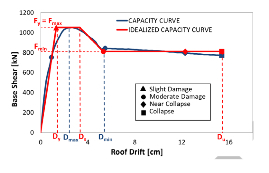
\includegraphics[width=10cm]{./figures/quadrilinearDF.jpg}
\caption{Multilinear capacity curve and parameters for the definition of R-$\mu$ relation.}
\label{fig:quadrilinear_DF}
\end{figure}

On the median "ida curve" the $\mu$-R pairs corresponding to the limit states (R$_{ds}$ and $\mu_{ds}$) can be found and turned into median spectral acceleration values for that limit state $\hat{S}_a$, to be used in equation \ref{eq:basic_DF}.

Once median $\hat{R}_{ds}$ and $\hat{\mu}_{ds}$ are found, the 84$^{th}$ and 16$^{th}$ fractiles of $\mu$ are extracted using top displacement record-to-record dispersion $\sigma_{ln(d_{roof})}$ from equation \ref{eq:beta_eq_RGM}, by Ruiz-Garcia and Miranda (2007). The steps to derive $\mu_{16\%}$ and $\mu_{84\%}$ are the following:
 
\begin{equation}
ln(d_{roof})_{16\%} = ln(\hat{d_{roof}})-\sigma_{ln(d_{roof})}
\end{equation}
\begin{equation}
ln(d_{roof})_{84\%} = ln(\hat{d_{roof}})+\sigma_{ln(d_{roof})}
\end{equation}
\begin{equation}
\mu_{16\%} = \hat{\mu} \exp{-\sigma_{ln(d_{roof})}}
\end{equation}
\begin{equation}
\mu_{84\%} = \hat{\mu} \exp{\sigma_{ln(d_{roof})}}
\end{equation}

Given the linear relationship between R and $\mu$, the R$_{16\%}$ and R$_{84\%}$ values at $\mu_{ds}$ are just linearly interpolated, and the record-to-record dispersion of the spectral acceleration $\beta_{S_{a, d}}$ at each $\mu_{ds}$ coincides with the dispersion of R, computed from the percentiles values, as in the following equation:

\begin{equation}
\label{eq:beta_DF}
\beta_{S_{a, d}} = \beta_{R(\mu)} = \frac{\ln R(\mu)_{84\%} - \ln R(\mu)_{16\%}}{2}
\end{equation} 

If dispersion due to uncertainty in the limit state definition $\beta_{\theta c}$ is different from zero it can be combined with the record-to-record dispersion $\beta_{\theta d}$ either in a simplified way or with a Monte Carlo sampling procedure similar to what is done in section \ref{subsubsec:single-building}.\\

In the simplified method the dispersion of $S_a$ due to uncertainty in the damage state threshold $\beta_{S_{a, c}}$  can be found converting the dispersion on the damage threshold $\beta_{\theta c}$, as explaind in section \ref{subsubsec:single-building} and reported in the following equation:

\begin{equation}
\beta_{S_{a c}} = \frac{1}{b} \beta_{\theta c}
\label{eq:betasc_DF}
\end{equation}

In order to derive the b values, which represent the slope of the R-$\mu$ relation in the log-space, a further step needs to be made, because the R-$\mu$-T is suggested by the authors as conservative, since it is not based on the median but on the mean $\mu$ given R. An attempt was made to correct it reducing the median R curve by 15\%, $\hat{R}_{corrected}$, as shown in equation \ref{eq:Rcorrected}, and extrapolating the corresponding $\hat{\mu}_{corrected}$.

\begin{equation}
\hat{R}_{corrected}=0.85\hat{R}
\label{eq:Rcorrected}
\end{equation}
\begin{equation}
b = \frac{ln(\hat{\mu}_{corrected})}{ln(\hat{R}_{corrected})}
\label{eq:bcorrected_DF}
\end{equation}

Finally the dispersion of $S_a$ due to record-to-record variability, can be combined with the dispersion of $S_a$ due to uncertainty in the damage state threshold, as in the following equation:

\begin{equation}
\beta_{S_a} = \sqrt{\beta_{S_{a, c}}^2+\beta_{S_{a, d}}^2}
\label{eq:betatot_DF}
\end{equation}

In the Monte Carlo approach different values of ductility limit state are now sampled from the lognormal distribution with median the median value of the ductility limit state, and dispersion the input $\beta_{\theta c}$. For each of these ductilities the corresponding $\hat{R}$, $R_{16\%}$, and $R_{84\%}$ values are found interpolating the aforementioned ida curves, and converted into $\hat{S}_{a,ds}$ and $\beta_{\theta d}$ according to the equations \ref{eq:SaR} and \ref{eq:betaR}.
N random S$_a$ for each of the N sampled ductility limit states are computed using $\hat{S}_{a,ds}$ and $\beta_{\theta d}$, and their median and the dispersion are estimated. These parameters constitute the median $\hat{S}_{a,ds}$ and the total dispersion $\beta_{S_a}$ for the considered damage state. The procedure is repeated for each damage state.\\

To derive a discrete vulnerability function at certain intensity measure levels, the input damage-to-loss factors are applied to the probability of occurance of each damage state, extracted from the probability of exceedance of each damage state described by the fragility function. A value of loss ratio is thus defined for the vector of selected intensity measure levels.

\subsubsection{Multiple Building Fragility and Vulnerability function}
\label{subsubsec:multiple-building-DF}
 If multiple buildings have been input to derive fragility function for a class of buildings all $\hat{S}_{a, blg}$ and $\beta_{S_a, blg}$ are combined in a single lognormal curve as described in section \ref{subsubsec:multiple-buildings}. The same holds for vulnerability function, as described in the same section.

\subsubsection{Inputs}
The data the user needs provided and the their format is described in section \ref{subsubsec:InputSpo2ida}

\subsubsection{Calculation Steps to be changed} 
The overall workflow of R-$\mu$-T-based procedure is summarised in this section. The option \textit{an\_type} must be set equal to 2 and the option \textit{in\_type} according to the input at disposal. The corresponding inputs should follow the requirements described in section \ref{subsubsec:InputSpo2ida}. At this point the code proceeds with the following steps:

\begin{enumerate}
\item 
\begin{enumerate}
\item If \textit{in\_type} = 0, the roof displacement at each limit state and the idealised pushover curve parameters are extracted from \textit{displacement\_profile.csv} and \textit{idealised\_curve.csv} respectively.

\item If \textit{in\_type} = 1 the results from a pushover analysis are extracted from \textit{displacements\_pushover.csv} and \textit{reactions\_pushover.csv} and drift limit states from {limits.csv}. The idealised pushover curve is then derived in the \textit{idealisation} function, where the idealisation process is conducted according to the Gem Analytical Vulnerability Guidelines.	\end{enumerate}

\item The csv input files are parsed with the function \textit{read\_data} according to the defined options. The parameters essential to the analysis are return together with a graphical visualisation of the inputs if the variable \textit{plotflag}[0] is equal to 1.

\item The parameters extracted are used in the \textit{DFfragility} function, within the \textit{fragility\_process} function, to derive ductility levels $\mu_{ds}$, median spectral acceleration $\hat{S}_{a,ds}$ and the total dispersion $\beta_{S_a}$ at each limit state through the following steps:
\begin{itemize}
\item The idealised MDoF system is transformed into an equivalent SDoF system, using $\Gamma_1$.
\item Ductility levels $\mu_{ds}$ corresponding to each damage threshold, are defined.
\item R and C$_R$ are computed, using eq. \ref{eq:mu_DF} and \ref{eq:Cr_DF} respectively.
\item $\hat{S}_{a,ds}$ and the corresponding dispersion  $\beta_{S_{a, d}}$ are computed using eq. \ref{eq:basic_DF} and \ref{eq:beta_DF} respectively.
\item R$_{corrected}$ curve are found reducing by 15\% the median R curve, and the corresponding $\mu_{corrected}$ corrected are extrapolated.
\item b value is found from R and $\mu$ according to eq. \ref{eq:bcorrected_DF}.

\begin{enumerate}
\item If the variable \textit{MC} = 0 uncertainty in the model is expressed in terms of dispersion in S$_a$ $\beta_{S_{a, c}}$ according to eq. \ref{eq:betasc_DF} and combined with $\beta_{S_{a, d}}$ to get the total dispersion $\beta_{S_a}$, using eq. \ref{eq:betatot_DF}.
\item If the variable \textit{MC} is different from 0 different ductility limit states are sampled for each median ductility level $\mu_{ds}$ and for each of these MC values of $\hat{S}_{a,ds}$ and $\beta_{S_{a, d}}$ are computed, as described in section \ref{subsubsec:single-building-DF}. Their median and the dispersion are estimated. These parameters constitute the median $\hat{S}_{a,ds}$ and the total dispersion $\beta_{S_a}$ for the considered damage state. 
\end{enumerate}

\item All $\hat{S}_{a, ds}(T_1)$ are converted to mean $\mu_{ln(S_{a, ds})}(T_1)$ and then to the intensity measure in common with the rest of the buildings, $\mu_{ln(S_{a, ds}(T_{av}))}$, according to eq. \ref{eq:Sa(Tav)}.
\end{itemize}

\item Step 2. and 3. are repeated for the number of input buildings.

\item
\begin{enumerate}

\item If \textit{vuln} = 0: All $\hat{S}_{a,ds}$ and $\beta_{S_{a, d}}$ from all the buildings and all the sampled ductility limit states are combined in a single lognormal curve, as described in section \ref{subsubsec:single-building-spo2ida}. 
Mean $\mu_{ln(S_{a})}$ and total dispersion $\beta_{S_a}$ are then converted to logarithmic mean $\mu_{S_a}$ and logarithmic covariance $cov_{S_a}$, according to equations \ref{eq:median-to-mean} and \ref{eq:dispersion-to-standard} respectively.
Fragility curves for the class of buildings are displayed if the variable \textit{plotflag}[2] = 1, and logarithmic $\mu_{S_a}$ and $cov_{S_a}$ are exported in the \textit{outputs} folder.

\item If \textit{vuln} =1:  
For the intensity measure levels defined in the variable \textit{iml} a value of loss ratio $\mu_{LR, iml, blg}$ is defined for each building and a standard deviation $\sigma_{LR, iml, blg}$, if dispersion due to uncertainty in the limit state $\beta_{\theta c}$ is different from zero. They are finally combined in a single mean and standard deviationas described in section \ref{subsubsec:multiple-building-spo2ida}. Vulnerability curve for the class of buildings is displayed if the variable \textit{plotflag}[3] = 1, and $\mu_{LR}$ and $cov_{LR}$ at each iml are exported in the \textit{outputs} folder.
\end{enumerate}

\end{enumerate}

		\subsection{NLS methods without record-to-record dispersion}
		\label{subsec:nls-no-dispersion}
		Still to implement

	\section{Non-linear Dynamic (NLD) Methods}
	\label{sec:nld-intro}
	Nonlinear Dynamic Methods are based on the results of many dynamic analyses, which relate the seismic response of a structure, represented by an Engineering Demand Parameter (EDP), like maximum top displacement, maximum inter-storey drift ratio, maximum top drift etc., to the Intensity Measure Level (IML) of the input accelerograms. 
Many methods exists in literature to perform a series of dynamic analysis and to post-process the results in order to derive fragility curves. Some of them treat a single building to estimate directly the median seismic intensity value corresponding to the attainment of different damage state thresholds (limit states), and the corresponding dispersion (Vamvatsikos and Cornell, 2002, Ellingwood and Kinali, 2009). Others treat a class of buildings, and lead to the evaluation of the probabilities of different damage states for a series of IMLs and thus to the set up of a damage probability matrix (Singhal and Kiremidjian, 1996, Silva et al., 2013).

The former approach has been implemented in the Ida-based procedure and explained in section \ref{subsec:nld-ida}, the latter in the DPM-based procedure, explained in section \ref{subsec:nld-dpm}. Both sections contains the necessary scientific background behind the code and their step-by-step implementation in the python script.

		\subsection{Using the NLD module}
		\label{subsec:nld-how-to-use}
		To start using the nonlinear dynamic method a command line text editor should be used to enter manually the folder location where the RMTK has been saved. The user should add the path \textit{/RMTK/Vulnerability/NDP}, where the nonlinear dynamic method script is located, as shown in the example below:

\begin{Verbatim}[frame=single, commandchars=\\\{\}, samepage=true]
cd path/to/rmtk/folder/RMTK
\end{Verbatim}

From the text editor iPython browser page can be opened with the following command line:

\begin{Verbatim}[frame=single, commandchars=\\\{\}, samepage=true]
ipython-2.7 notebook --pylab=inline
\end{Verbatim}

Once the iPython page is opened on the browser, the python scripts contained in the RMTK directory will be visible. The file \textit{NDM.ipynb} should be selected to start the calculations.

In the initial section of the script "Define Options" the user needs to set the options and to enter the input corresponding to the defined options in the folder \textit{NDP/input}. In section~\ref{subsec:NDMoptions} the alternatives values that the initial variables can assume and their meaning are described in detail, while the parameters to be inserted in the input files are fully described in section~\ref{subsec:NDMinputs}.

		\subsection{Damage probability matrix DPM-based procedure}
		\label{subsec:nld-dpm}
		This procedure performs the post-processing part of a set of dynamic analyses to first assemble a damage probability matrix, and then use this data for the derivation of a fragility function. Therefore the results of a set of dynamic analyses previously run have to be input to start the process. A list of intensity measure associated to each accelerogram, and corresponding EDP for each structure of the building class can be input, along with the set of limit states expressed in terms of the same EDP. The EDPs resulting from the dynamic analyses are compared with the limit state displacements and a global damage state is assigned to each structure. Thus, for each record, the number of frames in each damage state can be obtained. The distribution of buildings in each damage state is organised in the damage probability matrix, with a number of rows equal to the number of ground motion records and a number of columns equal to the number of damage states.

The processing of the data continue with the estimation of the cumulative fraction of structures in each damage state, summing the percentages of frames belonging to all the subsequent damage states. A lognormal cumulative distribution function, expressing the probability of exceeding each damage state in a continuous fashion, is then fit to these results, leading to the statistical parameters of the fragility curves. The regression analysis is carried out using the maximum likelihood method.

This function have the advantage of accounting for the record-to-record variability by the use of many ground motion records, and the inter-building variability subjecting to the same set of accelerograms hundreds of structures representing the entire building class.

To derive a discrete vulnerability function at certain intensity measure levels, the input damage-to-loss factors are applied to the probability of occurance of each damage state, extracted from the probability of exceedance of each damage state described by the fragility function. For the vector of selected intensity measure levels a value of loss ratio is thus defined.

\subsubsection{Options}
\label{subsubsec:NDMoptions}
In the Options the user has to define first of all the type of inputs at disposal, setting the variable \textit{in\_ type}, choosing between entering a damage count matrix, which corresponds to a damage probability matrix, where the probabilities of each damage state are substituted by the count of buildings in that damage state, or IML and corresponding EDPs for each dynamic analysis

\begin{Verbatim}[frame=single, commandchars=\\\{\}, samepage=true]
in\_type = 0 # damage count matrix 
in\_type = 1# IMLs and EDPs 
\end{Verbatim}

The variable \textit{vulnerability} instead gives the opportunity to decide the type of outputs, whether to stop the process at the derivation of the fragility curves, or to go all the way up to the vulnerability curve definition, applying damage-to-loss functions.

\begin{Verbatim}[frame=single, commandchars=\\\{\}, samepage=true]
vulnerability = 0 # derive fragility curves 
vulnerability = 1 # derive vulnerability curve
\end{Verbatim}

The variable \textit{iml} is a numpy array that identifies the intensity measure levels for which loss ratios are computed and provided in the vulnerability curve.

\begin{Verbatim}[frame=single, commandchars=\\\{\}, samepage=true]
iml = np.linspace(0.1,15,100)
\end{Verbatim}

The variable \textit{plotflag} allows or inhibits the displaying of plots. It is a python list composed of 2 integers, each one controlling a different plot: fragility and vulnerability function respectively. Each integer can take as value either zero or one, whether the corresponding graph has to be displayed or not:

\begin{Verbatim}[frame=single, commandchars=\\\{\}, samepage=true]
plotflag = [1, 1] # plot all the graphs
plotflag = [0, 0] # do not plot any graph
\end{Verbatim}

The following variables set some of the characteristics of the plots:
\begin{itemize}
\item IMlabel: list of one strings defining the IM on the x axis as ['Sa(Tel)-m/s$^{2}$']
\item linew: integer for defining lines width.
\item fontsize : fontsize used for labels, graphs etc.
\end{itemize}

\subsubsection{Inputs}
\label{subsubsec:NDMinputs}
The inputs must be formatted as comma-separated value files (.csv), and saved in the folder \textit{input}, contained in the NDP directory. If any other environment different from Windows is used make sure that the "comma separated values Windows" is selected as saving option when creating the input files.  

Two types of input can be entered, whether the results of the set of dynamic analyses performed have already been organised in a damage probability matrix for or not. In the former case the variable \textit{in\_type} should be set to 0 and the damage count matrix should be input in the csv file \textit{dcm.csv}. The first two columns refer to the number of record and the corresponding intensity measure level, the following columns report the number of buildings in each damage state, as shown in the following table:

\begin{table}[H]
\centering
\begin{tabular}{|c|c|c|c|c|} \hline
\textbf{n.records} & \textbf{Intensity Measure Level} & \textbf{DS$_0$} & \textbf{DS$_1$} & \textbf{DS$_2$} \\ \hline
1 & 49.852 &	30 &	16 &	54\\ \hline
2 & 47.056 &	54 &	15 &	31\\ \hline
3 & 33.012 &	59 &	10 &	31\\ \hline
4 & 82.125 &	24 &	26 &	50\\ \hline
... & ... & ... & ... & ... \\ \hline
5 & 37.499 &	58 &	5 &	37\\ \hline
\end{tabular}
\end{table}

In the latter case the variable \textit{in\_type} should be set to 1, and the results of the set of dynamic analyses should be entered in the \textit{edp.csv} file in the following fashion: number of record, corresponding IML, and corresponding EDPs for each building subjected to that record.

\begin{table}[H]
\centering
\begin{tabular}{|c|c|c|c|c|c|} \hline
\textbf{n.records} & \textbf{IML} & \textbf{edp$_{blg,1}$} & \textbf{edp$_{blg,2}$} & \textbf{...} & \textbf{edp$_{blg,n}$} \\ \hline
1 &	69.209 &	-0.00069 &	0.00031 & ... &	0.00131\\ \hline
2 &	75.470 &	0.00102 & 	0.00202 & ... &	0.00302\\ \hline
3 &	62.233 &	-0.00090 &	0.00010 & ... &	0.00110\\ \hline
4 &	168.47 &	-0.00246 &	-0.00146 & ... &	-0.00046\\ \hline
5 &	67.612 &	0.00095 & 	0.00195 & ... &	0.00295\\ \hline
... & ... & ... & ... & ... & ...\\ \hline
n &	34.484 &	0.00036 & 	0.00136 & ... & 	0.00236\\ \hline
\end{tabular}
\end{table}

In this case also the limit states must be input in the \textit{limits.csv} file. Each line of the file corresponds to the limit states of a building, but if all the buildings share the same limits a single line can be input.

\begin{table}[H]
\centering
\begin{tabular}{|c|c|c|c|c|} \hline
\textbf{n.building} & \textbf{LS$_1$} & \textbf{LS$_2$} & \textbf{LS$_3$} & \textbf{LS$_4$} \\ \hline
1 & 0.003 &	0.010 &	0.025 &	0.0337\\ \hline
2 & 0.004 &	0.015 &	0.020 &	0.035\\ \hline
3 & 0.002 &	0.019 &	0.027 &	0.032\\ \hline
... & ... & ... & ... & ...\\ \hline
n & 0.0024 &	0.016 &	0.025 &	0.03\\ \hline
\end{tabular}
\end{table}

\subsubsection{Calculations}
The overall workflow of the DPM-based procedure is summarised in this section. The option \textit{in\_type} should be set according to the input at disposal. The corresponding inputs should follow the requirements described in section \ref{subsubsec:inputs}. At this point the code proceeds with the following steps:

\begin{enumerate}
\item In the function \textit{read\_data} the inputs are read and the damage count matrix is returned.
\begin{enumerate}
\item If \textit{in\_type} = 0, the damage count matrix is extracted directly from the \textit{dcm.csv} file.

\item If \textit{in\_type} = 1 the IMLs of the records used in the dynamic analyses and the corresponding EDPs are extracted from \textit{edp.csv} and the limit states for each building, expressed in terms of the same EDP, are extracted from \textit{limits.csv}.	 These data are converted into a damage count matrix according to the method described in section~\ref{subsec:NDMtheory}.
\end{enumerate}

\item The parameters extracted are used to derive the Probability of Exceedance (PoE) of each limit state for each IML, as described in section~\ref{subsec:NDMtheory}.

\item The PoEs are fitted with a lognormal function using the maximum likelihood method. The mean $\mu_{ln IML}$ and standard deviation $\sigma_{ln IML}$ of the corresponding normal distribution for the entire class of buildings are found for each limit state.

\item The $\mu_{ln IML}$ and $\sigma_{ln IML}$ are converted to logarithmic $\mu_{IML}$ and $\sigma_{IML}$. The fragility curves for the class of buildings are displayed if the variable \textit{plotflag}[0] = 1, and the logarithmic $\mu_{IML}$ and $\sigma_{IML}$ are exported in the \textit{outputs} folder.

\item If vulnerability =1:  For the intensity measure levels defined in the variable \textit{iml} a value of loss ratio is defined, according to section \ref{subsec:NDMtheory}. A vulnerability curve for the class of buildings is displayed if the variable~\textit{plotflag}[1] = 1, and the loss ratios at each iml are exported in the \textit{outputs} folder.

\end{enumerate}

		\subsection{Post-processing IDA}
		\label{subsec:nld-ida}
		Post processing IDA

		% \subsection{Multiple stripe analysis (Jalayer, 2003)}
		% \label{subsec:nld-msa}
		% \input{./tex/nld-msa}

%----------------------------------------------------------------------------------------
%	BIBLIOGRAPHY
%----------------------------------------------------------------------------------------
% \chapter{Bibliography}
%\addcontentsline{toc}{chapter}{\textcolor{ocre}{Bibliography}}
\section{Books}
%\addcontentsline{toc}{section}{Books}
\printbibliography[heading=bibempty,type=book]
\section{Articles}
%\addcontentsline{toc}{section}{Articles}
\printbibliography[heading=bibempty,type=article]
\section{Other Sources}
%\addcontentsline{toc}{section}{Reports}
\printbibliography[heading=bibempty,nottype=book,nottype=article]


%----------------------------------------------------------------------------------------
%	INDEX
%----------------------------------------------------------------------------------------

\cleardoublepage
\phantomsection
\setlength{\columnsep}{0.75cm}
\addcontentsline{toc}{chapter}{\textcolor{ocre}{Index}}
\printindex
\printglossary


%----------------------------------------------------------------------------------------
%	APPENDICES
%----------------------------------------------------------------------------------------
%\part{Appendices}
\appendix
\chapterimage{./figures/chapter_head_2.pdf} % Chapter heading image
\chapter{The 10 Minute Guide to Python!}
\label{sec:python_guide}
% \begin{myfancybox}
% The objectives of this chapter are:
% \begin{itemize}
%     \item To introduce Python data types to facilitate use of the RMTK for Python beginners
% \end{itemize}
% \end{myfancybox}
The HMTK is intended to be used by scientists and engineers without the necessity of having an existing knowledge of Python. It is hoped that the examples contained in this manual should provide enough context to allow the user to understand how to use the tools for their own needs. In spite of this, however, an understanding of the fundamentals of the Python programming language can greatly enhance the user experience and permit the user to join together the tools in a workflow that best matches their needs. 

The aim of this appendix is therefore to introduce some fundamentals of the Python programming language in order to help understand how, and why, the HMTK can be used in a specific manner. If the reader wishes to develop their knowledge of the Python programming language beyond the examples shown here, there is a considerable body of literature on the topic from both a scientific and developer perspective.

\section{Basic Data Types}

Fundamental to the use of the HMTK is an understanding of the basic data types Python recognises:


\subsection{Scalar Parameters}

\begin{itemize}
\item \textbf{float} A floating point (decimal) number. If the user wishes to enter in a floating point value then a decimal point must be included, even if the number is rounded to an integer.

\begin{python}[frame=single]
>> a = 3.5
>> print a, type(a)
3.5 <type 'float'>
\end{python}

\item \textbf{integer} An integer number. If the decimal point is omitted for a floating point number the number will be considered an integer

\begin{python}[frame=single]
>> b = 3
>> print b, type(b)
3 <type 'int'>
\end{python}

The functions \verb=float()= and \verb=int()= can convert an integer to a float and vice-versa. Note that taking \verb=int()= of a fraction will round the fraction down to the nearest integer

\begin{python}[frame=single]
>> float(b)
3
>> int(a)
3
\end{python}

\item \textbf{string} A text string (technically a ``list'' of text characters). The string is indicated by the quotation marks ''something'' or 'something else'

\begin{python}[frame=single]
>> c = "apples"
>> print c, type(c)
apples <type 'str'>
\end{python}

\item \textbf{bool} For logical operations python can recognise a variable with a boolean data type (\verb=True= / \verb=False=).

\begin{python}[frame=single]
>> d = True
>> if d:
       print "y"
   else:
       print "n"
y
>> d = False
>> if d:
       print "y"
   else:
       print "n"
n
\end{python}

\emph{Care should be taken in Python as the value 0 and 0.0 are both recognised as False if applied to a logical operation. Similarly, booleans can be used in arithmetic where True and False take the values 1 and 0 respectively}

\begin{python}[frame=single]
>> d = 1.0
>> if d:
       print "y"
   else:
       print "n"
y
>> d = 0.0
>> if d:
       print "y"
   else:
       print "n"
n
\end{python}
\end{itemize}

\subsubsection{Scalar Arithmetic}

Scalars support basic mathematical operations (\# indicates a comment):

\begin{python}[frame=single]
>> a = 3.0
>> b = 4.0
>> a + b # Addition
7.0
>> a * b # Multiplication
12.0
>> a - b # Subtraction
-1.0
>> a / b # Division
0.75
>> a ** b  # Exponentiation
81.0
# But integer behaviour can be different!
>> a = 3; b = 4
>> a / b
0
>> b / a
1
\end{python}

\subsection{Iterables}

Python can also define variables as lists, tuples and sets. These data types can form the basis for iterable operations. It should be noted that unlike other languages, such as Matlab or Fortran, Python iterable locations are zero-ordered (i.e. the first location in a list has an index value of 0, rather than 1). 

\begin{itemize}
\item \textbf{List} A simple list of objects, which have the same or different data types. Data in lists can be re-assigned or replaced
\begin{python}[frame=single]
>> a_list = [3.0, 4.0, 5.0]
>> print a_list
[3.0, 4.0, 5.0]
>> another_list = [3.0, "apples", False]
>> print another_list
[3.0, 'apples', False]
>> a_list[2] = -1.0
a_list = [3.0, 4.0, -1.0]
\end{python}

\item \textbf{Tuples} Collections of objects that can be iterated upon. As with lists, they can support mixed data types. However, objects in a tuple cannot be re-assigned or replaced.
\begin{python}[frame=single]
>> a_tuple = (3.0, "apples", False)
>> print a_tuple
(3.0, 'apples', False)
# Try re-assigning a value in a tuple
>> a_tuple[2] = -1.0
TypeError                Traceback (most recent call last)
<ipython-input-43-644687cfd23c> in <module>()
----> 1 a_tuple[2] = -1.0

TypeError: 'tuple' object does not support item assignment
\end{python}

\item \textbf{Range} A range is a convenient function to generate arithmetic progressions. They are called with a \verb=start=, a \verb=stop= and (optionally) a \verb=step= (which defaults to 1 if not specified)

\begin{python}[frame=single]
>> a = range(0, 5)
>> print a
[0, 1, 2, 3, 4]  # Note that the stop number is not 
                 # included in the set!  
>> b = range(0, 6, 2)
>> print b
[0, 2, 4]
\end{python}

\item \textbf{Sets} A set is a special case of an iterable in which the elements are unordered, but contains more enhanced mathematical set operations (such as intersection, union, difference, etc.)

\begin{python}[frame=single]
>> from sets import Set
>> x = Set([3.0, 4.0, 5.0, 8.0])
>> y = Set([4.0, 7.0])
>> x.union(y)
Set([3.0, 4.0, 5.0, 7.0, 8.0])
>> x.intersection(y)
Set([4.0])
>> x.difference(y)
Set([8.0, 3.0, 5.0]) # Notice the results are not ordered!
\end{python}
\end{itemize}

\subsubsection{Indexing}

For some iterables (including lists, sets and strings) Python allows for subsets of the iterable to be selected and returned as a new iterable. The selection of elements within the set is done according to the \verb=index= of the set. 

\begin{python}[frame=single]
>> x = range(0, 10)  # Create an iterable
>> print x
[0, 1, 2, 3, 4, 5, 6, 7, 8, 9]
>> print x[0] # Select the first element in the set
0             # recall that iterables are zero-ordered!
>> print x[-1] # Select the last element in the set
9
>> y = x[:] # Select all the elements in the set
>> print y
[0, 1, 2, 3, 4, 5, 6, 7, 8, 9]
>> y = x[:4]  # Select the first four element of the set
>> print y
[0, 1, 2, 3]
>> y = x[-3:] # Select the last three elements of the set
>> print y
[7, 8, 9]
>> y = x[4:7] # Select the 4th, 5th and 6th elements
>> print y
[4, 5, 6]
\end{python}

\subsection{Dictionaries}

Python is capable of storing multiple data types associated with a map of variable names inside a single object. This is called a ``Dictionary'', and works in a similar manner to a ``data structure'' in languages such as Matlab. Dictionaries are used frequently in the HMTK as ways of structuring inputs to functions that share a common behaviour but may take different numbers and types of parameters on input.

\begin{python}[frame=single]
>> earthquake = {"Name": "Parkfield",
                 "Year": 2004,
                 "Magnitude": 6.1,
                 "Recording Agencies" = ["USGS", "ISC"]}
# To call or view a particular element in a dictionary
>> print earthquake["Name"], earthquake["Magnitude"]
Parkfield 6.1
\end{python}

\subsection{Loops and Logicals}

Python's syntax for undertaking logical operations and iterable operations is relatively straightforward.

\subsubsection{Logical}

A simple logical branching structure can be defined as follows:

\begin{python}[frame=single]
>> a = 3.5
>> if a <= 1.0:
       b = a + 2.0
   elif a > 2.0:
       b = a - 1.0
   else:
       b = a ** 2.0
>> print b
2.5
\end{python}

Boolean operations can are simply rendered as \verb=and=, \verb=or= and \verb=not=.
\begin{python}[frame=single]
>> a = 3.5
>> if (a <= 1.0) or (a > 3.0):
       b = a - 1.0
   else:
       b = a ** 2.0
>> print b
2.5
\end{python}

\subsubsection{Looping}

There are several ways to apply looping in python. For simple mathematical operations, the simplest way is to make use of the \textbf{range} function:

\begin{python}[frame=single]
>> for i in range(0, 5):
       print i, i ** 2
0  0
1  1
2  4
3  9
4  16
\end{python}

The same could be achieved using the \verb=while= function (though possibly this approach is far less desirable depending on the circumstance):

\begin{python}[frame=single]
>> i = 0
>> while i < 5:
       print i, i ** 2
       i += 1
0  0
1  1
2  4
3  9
4  16
\end{python}

A \verb=for= loop can be applied to any iterable:

\begin{python}[frame=single]
>> fruit_data = ["apples", "oranges", "bananas", "lemons", 
                 "cherries"]
>> i = 0
>> for fruit in fruit_data:
       print i, fruit
       i += 1
0  apples
1  oranges
2  bananas
3  lemons
4  cherries 
\end{python}

The same results can be generated, arguably more cleanly, by making use of the \verb=enumerate= function:

\begin{python}[frame=single]
>> fruit_data = ["apples", "oranges", "bananas", "lemons", 
                 "cherries"]
>> for i, fruit in enumerate(fruit_data):
       print i, fruit
0  apples
1  oranges
2  bananas
3  lemons
4  cherries 
\end{python}

As with many other programming languages, Python contains the statements \verb=break= to break out of a loop, and \verb=continue= to pass to the next iteration.

\begin{python}[frame=single]
>> i = 0
>> while i < 10:
       if i == 3:
           i += 1
           continue
       elif i == 5:
           break
       else:
           print i, i ** 2
       i += 1
0  0
1  1
2  4
4  16
\end{python}

\section{Functions}

Python easily supports the definition of functions. A simple example is shown below. \emph{Pay careful attention to indentation and syntax!}

\begin{python}[frame=single]
>> def a_simple_multiplier(a, b):
       """
       Documentation string - tells the reader the function 
       will multiply two numbers, and return the result and
       the square of the result
       """
       c = a * b
       return c, c ** 2.0

>> x = a_simple_multiplier(3.0, 4.0)
>> print x
(12.0, 144.0)
\end{python}

In the above example the function returns two outputs. If only one output is assigned then that output will take the form of a tuple, where the elements correspond to each of the two outputs. To assign directly, simply do the following:

\begin{python}[frame=single]
>> x, y = a_simple_multiplier(3.0, 4.0)
>> print x
12.0
>> print y
144.0
\end{python}

\section{Classes and Inheritance}

Python is one of many languages that is fully object-oriented, and the use (and terminology) of objects is prevalent throughout the HMTK and this manual. A full treatise on the topic of object oriented programming in Python is beyond the scope of this manual and the reader is referred to one of the many textbooks on Python for more examples

\subsection{Simple Classes}

A class is an object that can hold both attributes and methods. For example, imagine we wish to convert an earthquake magnitude from one scale to another; however, if the earthquake occurred after a user-defined year we wish to use a different formula. This could be done by a method, but we can also use a class:

\begin{python}[frame=single]
>> class MagnitudeConverter(object):
       """
       Class to convert magnitudes from one scale to another
       """
       def __init__(self, converter_year):
           """
           """
           self.converter_year = converter_year
       
       def convert(self, magnitude, year):
           """
           Converts the magnitude from one scale to another
           """
           if year < self.converter_year:
               converted_magnitude = -0.3 + 1.2 * magnitude
           else:
               converted_magnitude = 0.1 + 0.94 * magnitude
           return converted_magnitude
                  
>> converter1 = MagnitudeConverter(1990)
>> mag_1 = converter1.convert(5.0, 1987)
>> print mag_1
5.7
>> mag_2 = converter1.convert(5.0, 1994)
>> print mag_2
4.8
# Now change the conversion year
>> converter2 = MagnitudeConverter(1995)
>> mag_1 = converter2.convert(5.0, 1987)
>> print mag_1
5.7
>> mag_2 = converter2.convert(5.0, 1994)
>> print mag_2
5.7  
\end{python}

In this example the class holds both the attribute \verb=converter_year= and the method to convert the magnitude. The class is created (or ``instantiated'') with only the information regarding the cut-off year to use the different conversion formulae. Then the class has a method to convert a specific magnitude depending on its year.

\subsection{Inheritance}

Classes can be useful in many ways in programming. One such way is due to the property of inheritance. This allows for classes to be created that can inherit the attributes and methods of another class, but permit the user to add on new attributes and/or modify methods. 

In the following example we create a new magnitude converter, which may work in the same way as the \verb=MagnitudeConverter= class, but with different conversion methods.

\begin{python}[frame=single]
>> class NewMagnitudeConverter(MagnitudeConverter):
       """
       A magnitude converter using different conversion
       formulae
       """
       def convert(self, magnitude, year):
           """
           Converts the magnitude from one scale to another
           - differently!!!
           """
           if year < self.converter_year:
               converted_magnitude = -0.1 + 1.05 * magnitude
           else:
               converted_magnitude = 0.4 + 0.8 * magnitude
           return converted_magnitude
# Now compare converters
>> converter1 = MagnitudeConverter(1990)
>> converter2 = NewMagnitudeConverter(1990)
>> mag1 = converter1.convert(5.0, 1987)
>> print mag1
5.7
>> mag2 = converter2.convert(5.0, 1987)
>> print mag2
5.15
>> mag3 = converter1.convert(5.0, 1994)
>> print mag3
4.8
>> mag4 = converter2.convert(5.0, 1994)
>> print mag4
4.4    
\end{python}

\subsection{Abstraction}

Inspection of the HMTK code (\href{https://github.com/GEMScienceTools/hmtk}{https://github.com/GEMScienceTools/hmtk}) shows frequent usage of classes and inheritance. This is useful in our case if we wish to make available different methods for the same problem. In many cases the methods may have similar logic, or may provide the same types of outputs, but the specifics of the implementation may differ. Functions or attributes that are common to all methods can be placed in a ``Base Class'', permitting each implementation of a new method to inherit the ``Base Class'' and its functions/attributes/behaviour. The new method will simply modify those aspects of the base class that are required for the specific method in question. This allows functions to be used interchangeably, thus allowing for a "mapping" of data to specific methods. 

An example of abstraction is shown using our two magnitude converters shown previously. Imagine that a seismic recording network (named "XXX") has a model for converting from their locally recorded magnitude to a reference global scale (for the purposes of narrative, imagine that a change in recording procedures in 1990 results in a change of conversion model). A different recording network (named ``YYY'') has a different model for converting their local magnitude to a reference global scale (and we imagine they also changed their recording procedures, but they did so in 1994). We can create a mapping that would apply the correct conversion for each locally recorded magnitude in a short catalogue, provided we know the local magnitude, the year and the recording network.

\begin{python}[frame=single]
>> CONVERSION_MAP = {"XXX": MagnitudeConverter(1990),
                     "YYY": NewMagnitudeConverter(1994)}
>> earthquake_catalogue = [(5.0, "XXX", 1985),
                           (5.6, "YYY", 1992),
                           (4.8, "XXX", 1993),
                           (4.4, "YYY", 1997)]
>> for earthquake in earthquake_catalogue:
       converted_magnitude = \ # Line break for long lines!
           CONVERSION_MAP[earthquake[1]].convert(earthquake[0],
                                                 earthquake[2])
       print earthquake, converted_magnitude
(5.0, "XXX", 1985) 5.7
(5.6, "YYY", 1992) 5.78
(4.8, "XXX", 1993) 4.612
(4.4, "YYY", 1997) 3.92
\end{python}

So we have a simple magnitude homogenisor that applies the correct function depending on the network and year. It then becomes a very simple matter to add on new converters for new agencies; hence we have a ``toolkit'' of conversion functions!

\section{Numpy/Scipy}

Python has two powerful libraries for undertaking mathematical and scientific calculation, which are essential for the vast majority of scientific applications of Python: Numpy (for multi-dimensional array calculations) and Scipy (an extensive library of applications for maths, science and engineering). Both libraries are critical to both OpenQuake and the HMTK. Each package is so extensive that a comprehensive description requires a book in itself. Fortunately there is abundant documentation via the online help for Numpy \href{www.numpy.org}{www.numpy.org} and Scipy \href{www.scipy.org}{www.scipy.org}, so we do not need to go into detail here. 

The particular facet we focus upon is the way in which Numpy operates with respect to vector arithmatic. Users familiar with Matlab will recognise many similarities in the way the Numpy package undertakes array-based calculations. Likewise, as with Matlab, code that is well vectorised is signficantly faster and more efficient than the pure Python equivalent. 

The following shows how to undertake basic array arithmetic operations using the Numpy library

\begin{python}[frame=single]
>> import numpy as np
# Create two vectors of data, of equal length
>> x = np.array([3.0, 6.0, 12.0, 20.0])
>> y = np.array([1.0, 2.0, 3.0, 4.0])
# Basic arithmetic
>> x + y   # Addition (element-wise)
np.array([4.0, 8.0, 15.0, 24.0])
>> x + 2   # Addition of scalar
np.array([5.0, 8.0, 14.0, 22.0])
>> x * y   # Multiplication (element-wise)
np.array([3.0, 12.0, 36.0, 80.0])
>> x * 3.0   # Multiplication by scalar
np.array([9.0, 18.0, 36.0, 60.0])
>> x - y   # Subtraction (element-wise)
np.array([2.0, 4.0, 9.0, 16.0])
>> x - 1.0   # Subtraction of scalar
np.array([2.0, 5.0, 11.0, 19.0])
>> x / y   # Division (element-wise)
np.array([3.0, 3.0, 4.0, 5.0])
>> x / 2.0   # Division over scalar
np.array([1.5, 3.0, 6.0, 10.0])
>> x ** y    # Exponentiation (element-wise)
np.array([3.0, 36.0, 1728.0, 160000.0])
>> x ** 2.0   # Exponentiation (by scalar)
np.array([9.0, 36.0, 144.0, 400.0])
\end{python}

Numpy contains a vast set of mathematical functions that can be operated on a vector (e.g.):

\begin{python}[frame=single]
>> x = np.array([3.0, 6.0, 12.0, 20.0])
>> np.exp(x)
np.array([2.00855369e+01, 4.03428793e+02, 1.62754791e+05,
         4.85165195e+08])
# Trigonometry
>> theta = np.array([0., np.pi / 2.0, np.pi, 1.5 * np.pi])
>> np.sin(theta)
np.array([0.0000, 1.0000, 0.0000, -1.0000])
>> np.cos(theta)
np.array([1.0000, 0.0000, -1.0000, 0.0000])
\end{python}

Some of the most powerful functions of Numpy, however, come from its logical indexing:

\begin{python}[frame=single]
>> x = np.array([3.0, 5.0, 12.0, 21.0, 43.0])
>> idx = x >= 10.0   # Perform a logical operation
>> print idx
np.array([False, False, True, True, True])
>> x[idx]   # Return an array consisting of elements
            # for which the logical operation returned True
np.array([12.0, 21.0, 43.0])
\end{python}

Create, index and slice n-dimensional arrays:

\begin{python}[frame=single]
>> x = np.array([[3.0,  5.0, 12.0, 21.0, 43.0],
                 [2.0,  1.0,  4.0, 12.0, 30.0],
                 [1.0, -4.0, -2.1,  0.0, 92.0]])
>> np.shape(x)
(3, 5)
>> x[:, 0]
np.array([3.0, 2.0, 1.0])
>> x[1, :]
np.array([2.0, 1.0, 4.0, 12.0, 30.0])
>> x[:, [1, 4]]
np.array([[ 5.0, 43.0],
          [ 1.0, 30.0],
          [-4.0, 92.0]])
\end{python}

The reader is referred to the online documentation for the full set of functions!





\end{document}